%Empieza configuracion de capitulo
\setstretch{1.0}
\titleformat{\chapter}[block]{\Large\bfseries}{CHAPTER \Huge\thechapter\vspace{25 pt}}{0 pt}{\\\fontsize{26}{36}\selectfont}
\titlespacing{\chapter}{0 pt}{30 pt}{50 pt}[0 pt]
\titleformat{\section}{\Large\bfseries}{\thesection}{0 pt}{\hspace{30 pt}}
\titleformat{\subsection}{\large\bfseries}{\thesubsection}{0 pt}{\hspace{30 pt}}
\pagestyle{fancy}
\fancyhead[LO,LE]{\footnotesize\emph{\leftmark}}
\fancyhead[RO,RE]{\thepage}
\fancyfoot[CO,CE]{}
%Termina configuracion de capitulo

\chapter{Experiments and Results}
\setstretch{1.5} %Regresa el interlineado a 1.5

\normalsize
\noindent

This section will describe the experiments we did in order to find the best
conditions for the embedded distributed system. We will describe each
experiment in the same order it was tested and explaining the reasons that make
us run that experiment.The variables that are involved are : 

\begin{itemize}
\item Run a simple sanity test in the embedded platform
\item Run the mpebch test suite in the embedded platform
\item Find out if chaning the OS for one custimized for the embedded platform
architecure (x86) give better results,
\item Find out the best implementation of MPI library and at the end, 
\item once that we have found the OS and MPI configuration that give better
performance results, we will apply this knowledge to solve a real application
where a distributed embedded system could improve the energy efficiency
\end{itemize}

\section{Run MPI sanity test in an embedded platform}

In order to find the enviroment that gives better performance of the MPIbench
tests, first is necesary to run the basic and simple MPI test. A simple code to
prove that the MPI implementation is working as espected is:

\begin{lstlisting}[frame=single,numbers=left,breaklines=true]
#include "mpi.h"
#include <stdio.h>
#include <stdlib.h>
#define  MASTER     0

int main (int argc, char *argv[])
{
    int   numtasks, taskid, len;
    char hostname[MPI_MAX_PROCESSOR_NAME];

    MPI_Init(&argc, &argv);
    MPI_Comm_size(MPI_COMM_WORLD, &numtasks);
    MPI_Comm_rank(MPI_COMM_WORLD,&taskid);
    MPI_Get_processor_name(hostname, &len);
    printf ("Hello from task % d on % s!\n", taskid, hostname);
    if (taskid == MASTER)
           printf("MASTER: Number of MPI tasks is: % d\n",numtasks);
    MPI_Finalize();

}
\end{lstlisting}

The way to compile it is: 

\begin{lstlisting}[frame=single,language=bash]
  $ mpicc -o mpi_hello_world mpi_hello_world.c
\end{lstlisting}


The way to run it is: 

\begin{lstlisting}[frame=single,language=bash]
  $ mpirun -n 4 -f host_file ./mpi_hello_world
\end{lstlisting}


After your program is compiled, it is ready to be executed. Now comes the part
where you might have to do some additional configuration. If you are running
MPI programs on a cluster of nodes, you will have to set up a host file. If you
are simply running MPI on a laptop or a single machine, disregard the next
piece of information.

The host file contains names of all of the computers on which your MPI job will
execute. For ease of execution, you should be sure that all of these computers
have SSH access, and you should also setup an authorized keys file to avoid a
password prompt for SSH. A simple host file looks like this.

\begin{lstlisting}[frame=single,language=bash]
  $ cat hostfile
    node1
    node2
    node3
\end{lstlisting}

Each one of these node is descrbed in an ssh file like this:

\begin{lstlisting}[frame=single,language=bash]
  $ cat ~/.ssh/config
    Host node1
        HostName node1-ip-or-hostname
        User user-of-the-ssh-key
        Port port-if-nedded
\end{lstlisting}

To run on a single system is not necesary to have a hostfile , however for our
experiments we will need more than one system.

The result of this experiment is as follows:

\begin{lstlisting}[frame=single,language=bash]
victor@minnow-1 tmp $ mpirun -n 4  ./hello
Hello from task 0 on minnow-1
MASTER: Number of MPI tasks is: 4
Hello from task 1 on minnow-1
Hello from task 2 on minnow-1
Hello from task 3 on minnow-1
\end{lstlisting}

After this experiment running on our embedded platform with a regular GNU/Linux
OS (Fedora), we prove that is possible to run MPI in an embedded system. But as
we know there are other options of GNU/Linux Operating Systems
(Suse/Debian/RedHat). Now the question is: Which one gives the best
performance under the MPIbenchs? . Before answering that quesiton is necesary
to answer the question: Is possible to run the MPbench under our system as well
as the hello world test we just did ?


\section{Run MPI benchmarks in an embedded platform}

The first aproach was to find out if is possible to run a sanity MPI test (MPI
hellow world) with a regular GNU Linux operating system under the embedded
system (Minnowboard\cite{minnowboard}),  From the list of suported GNU/Linux
based operatining system the minnowboad support, the one we selected was Fedora
\cite{fedora}.project. 


While MPBench can be run from the command line, it is designed to be run from
via the Makefile. Running it via the makefile automates the collection and
presentation process. The steps to run the benchmark are: 


\begin{lstlisting}[frame=single,language=bash]
victor@minnow-1 $ llcbench $ make linux-mpich
victor@minnow-1 $ llcbench $ make mp-bench
victor@minnow-1 $ llcbench $ make mp-run
\end{lstlisting}

After this last command the benchmark start to run under the Minnowboard, the
resutls are gather in a tar ball. The results can be ploted with gnuplot.
Gnuplot is a portable command-line driven graphing utility for Linux, OS/2, MS
Windows, OSX, VMS, and many other platforms. 

After the success of this experiment we can say that is possible to run the MPI
benchmarks on the embedded platoform with a regular Linux base operating system
(Fedora Project). now the ext question was: What if we change the operating
system? Can we get better numbers if we change the operating system?


\section{Test multiple operating systems to run the MPI benchmark}

We decided to use another Linux OS designed for Intel Architecture
/cite{clear-linux}.The Clear Linux Project for Intel Architecture is a
distribution built for various Cloud use cases. The project  want to showcase
the best of Intel Architecture technology, from low-level kernel features to
complex applications that span across the entire OS stack.

After running this two experiments we found interesting results that make us
think that maybe a much more custom OS could impprove the numbers of the MPI
benchmarks. These results are presented in the next figures:

\begin{figure}[H]
\centering
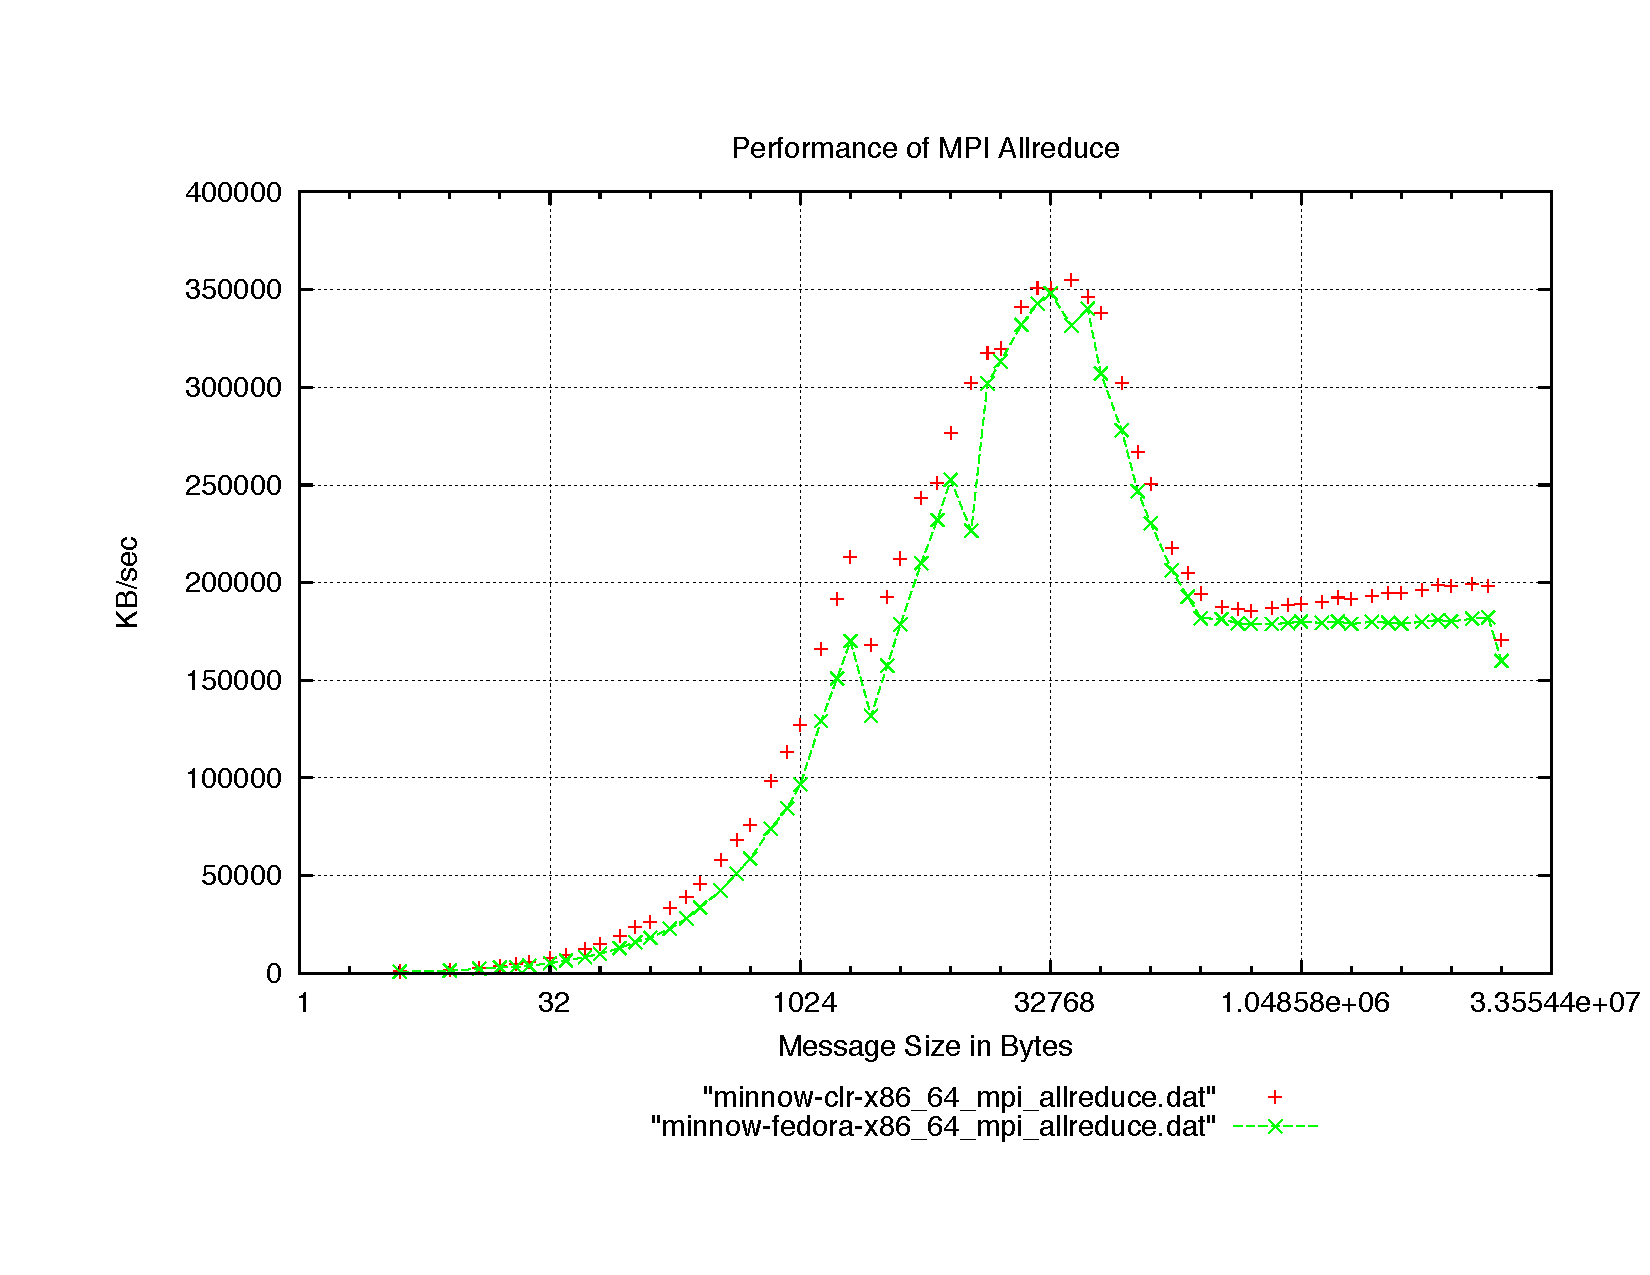
\includegraphics[width=0.75\textwidth]{images/mpbench_clr_experiments/mpi_allreduce.pdf}
\caption{MPI all reduce benchmark running in Minnowboard with Clear Linux and
Fedora (higher is better)}
\label{fig:5.1}
\end{figure}



\begin{figure}[H]
\centering
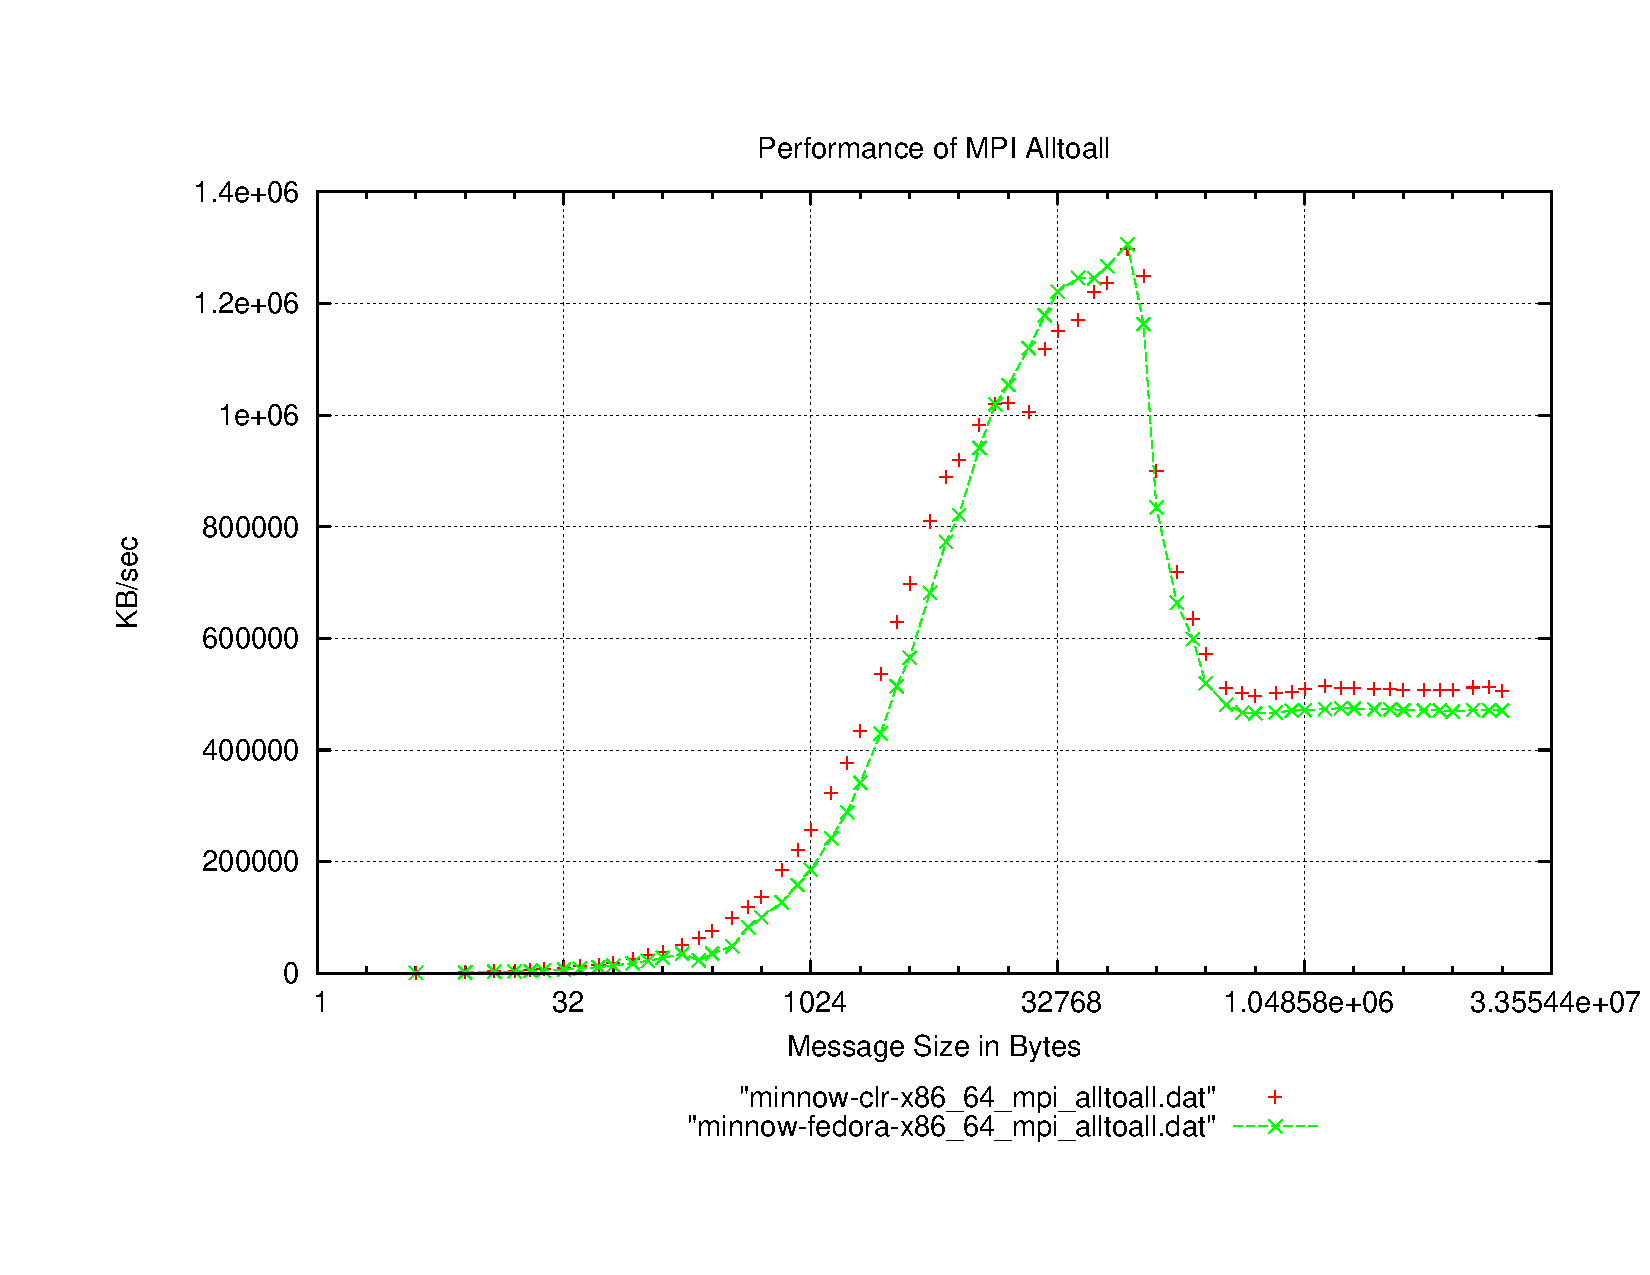
\includegraphics[width=0.75\textwidth]{images/mpbench_clr_experiments/mpi_alltoall.pdf}
\caption{MPI all to all benchmark running in Minnowboard with Clear Linux and
Fedora (higher is better)}
\label{fig:5.2}
\end{figure}


\begin{figure}[H]
\centering
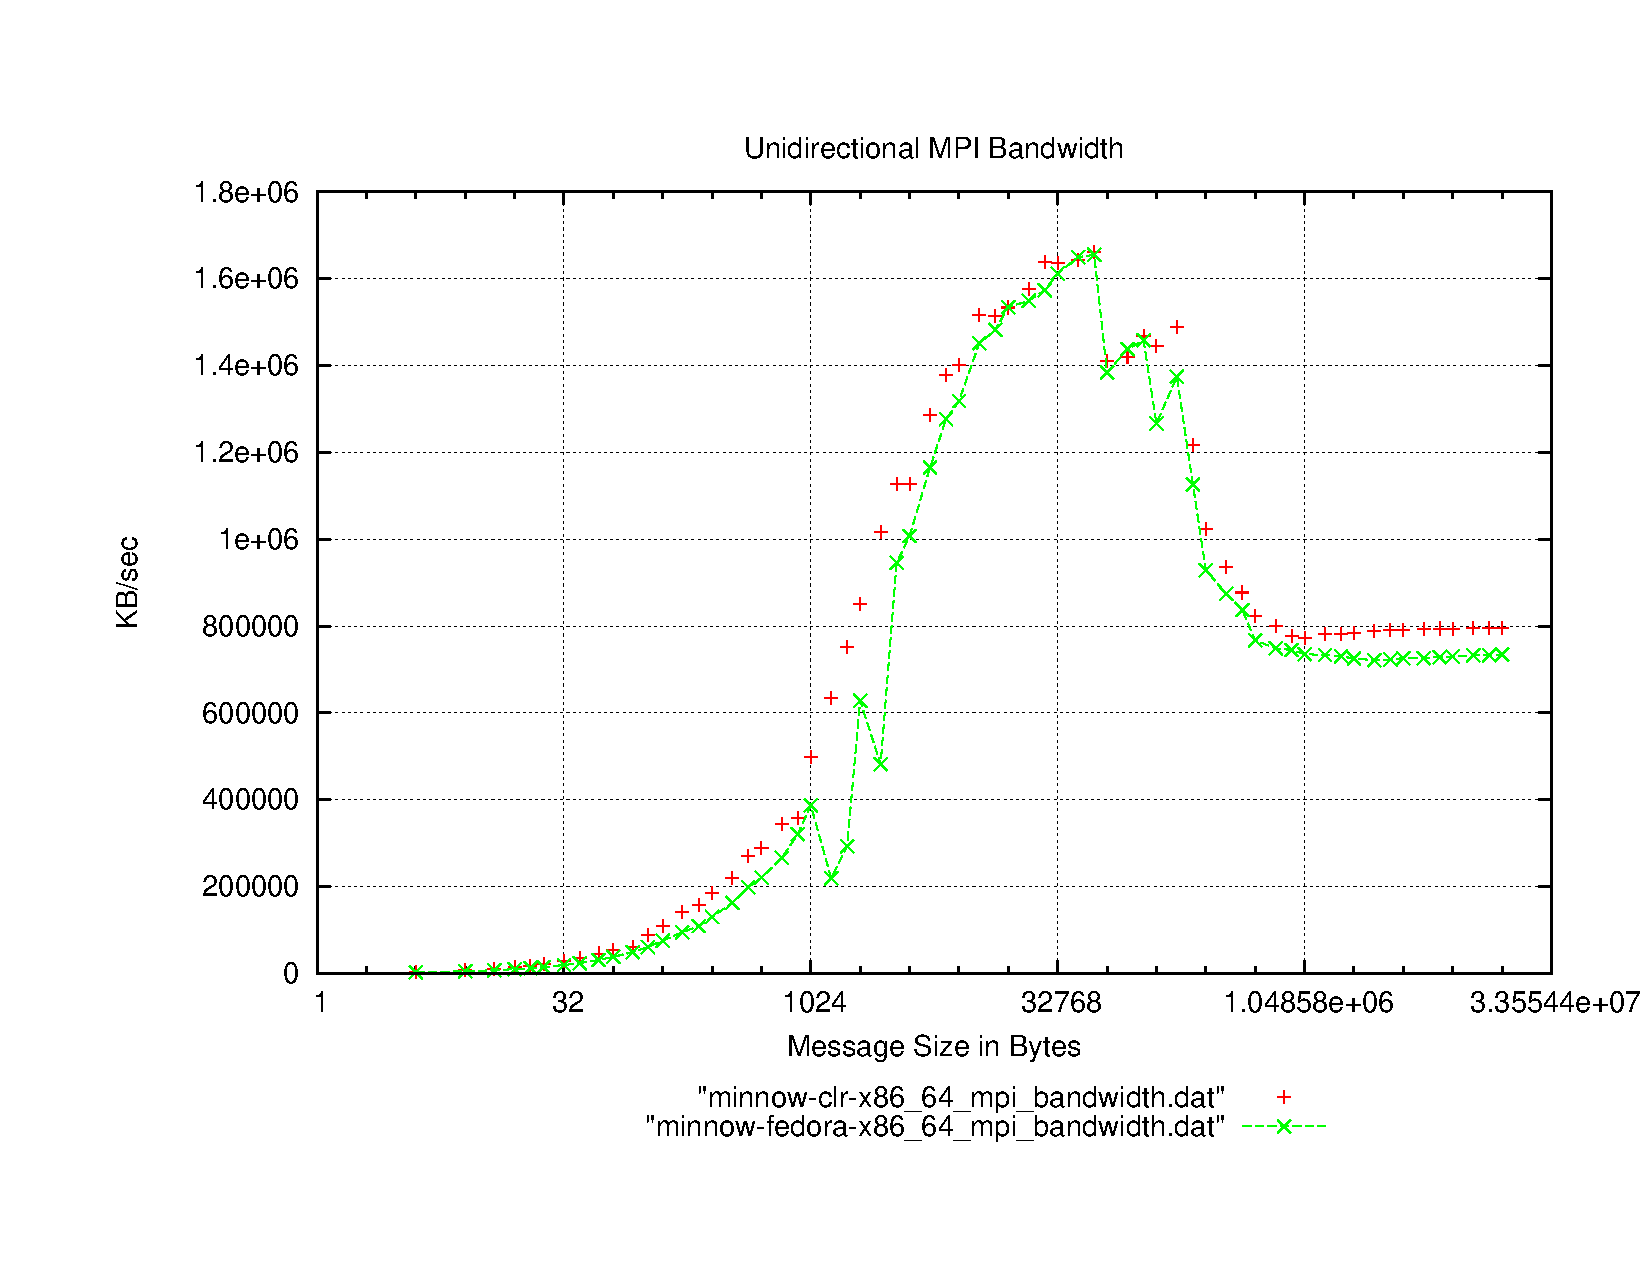
\includegraphics[width=0.75\textwidth]{images/mpbench_clr_experiments/mpi_bandwidth.pdf}
\caption{MPI bandwidth benchmark running in Minnowboard with Clear Linux and
Fedora (higher is better)}
\label{fig:5.3}
\end{figure}


\begin{figure}[H]
\centering
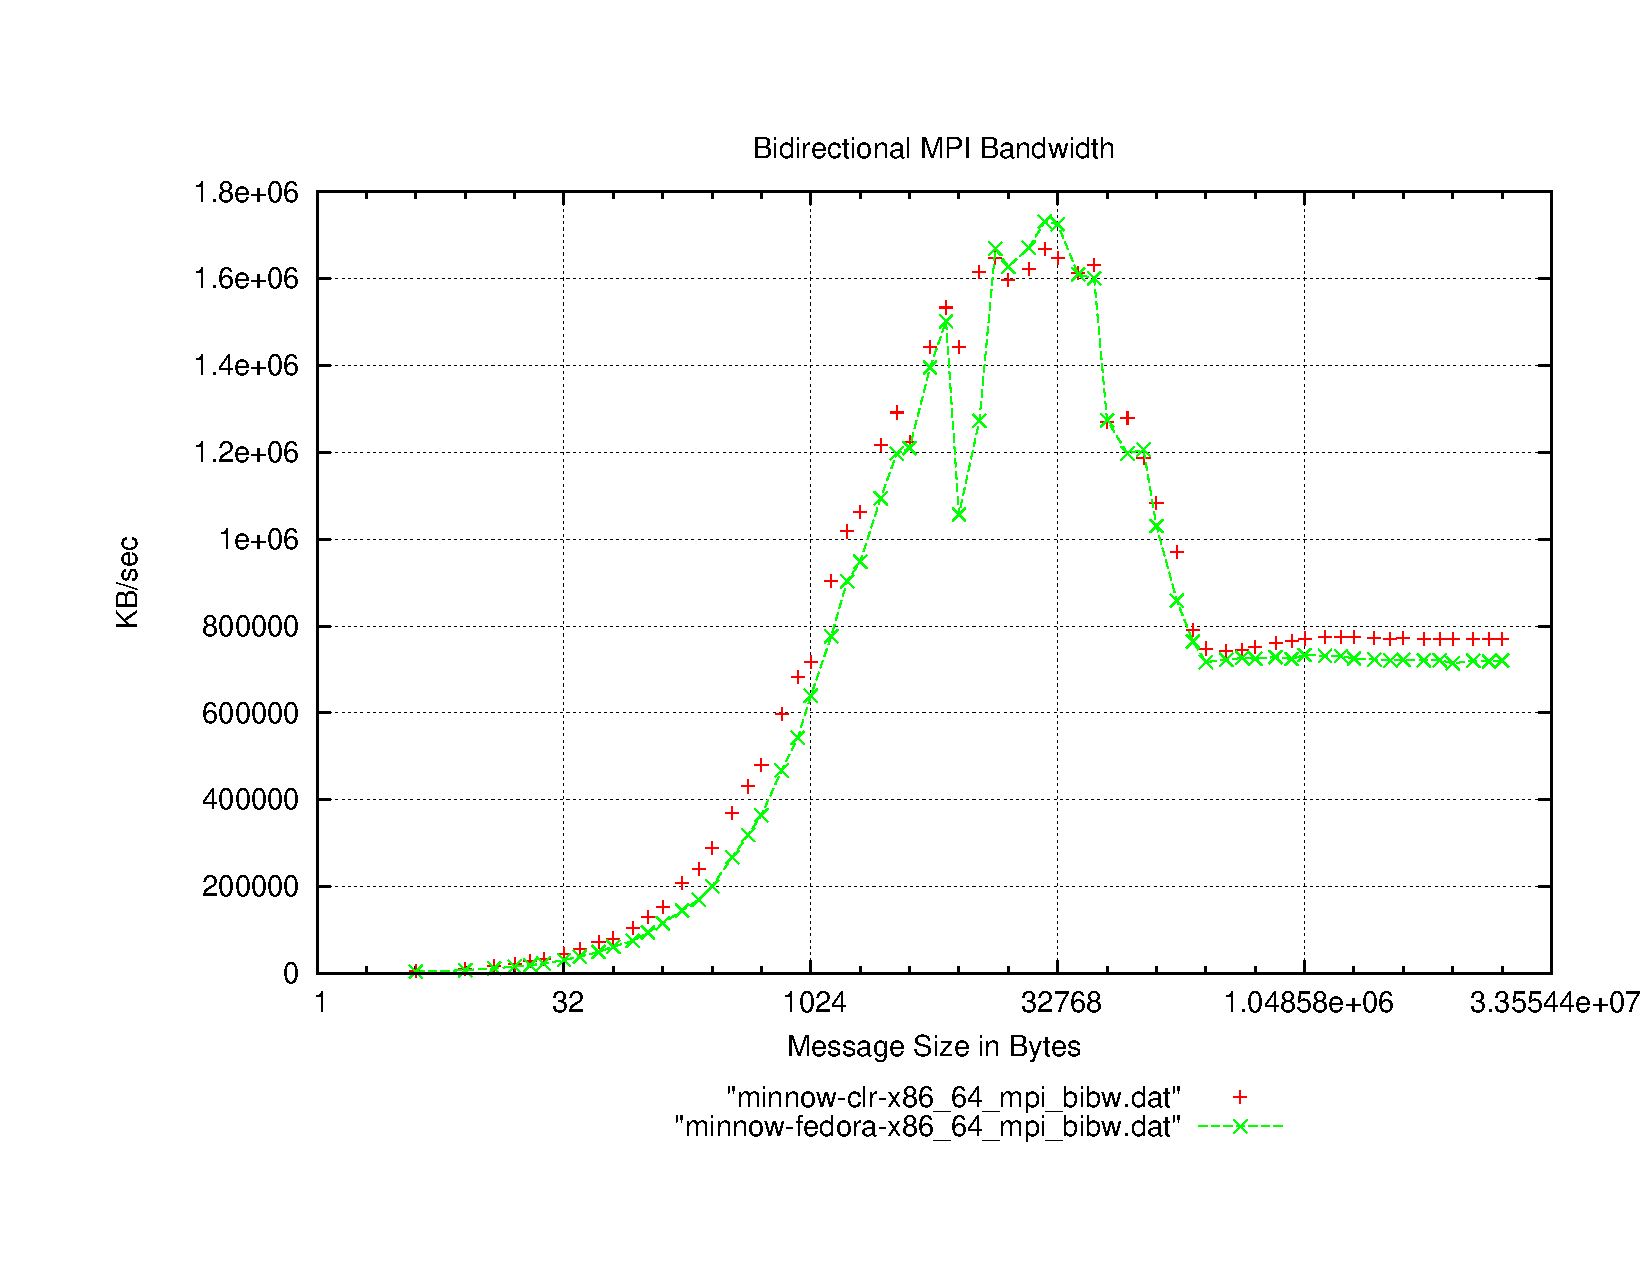
\includegraphics[width=0.75\textwidth]{images/mpbench_clr_experiments/mpi_bibw.pdf}
\caption{MPI Bi directional bandwidth running in Minnowboard with Clear Linux
and Fedora (higher is better)}
\label{fig:5.4}
\end{figure}


\begin{figure}[H]
\centering
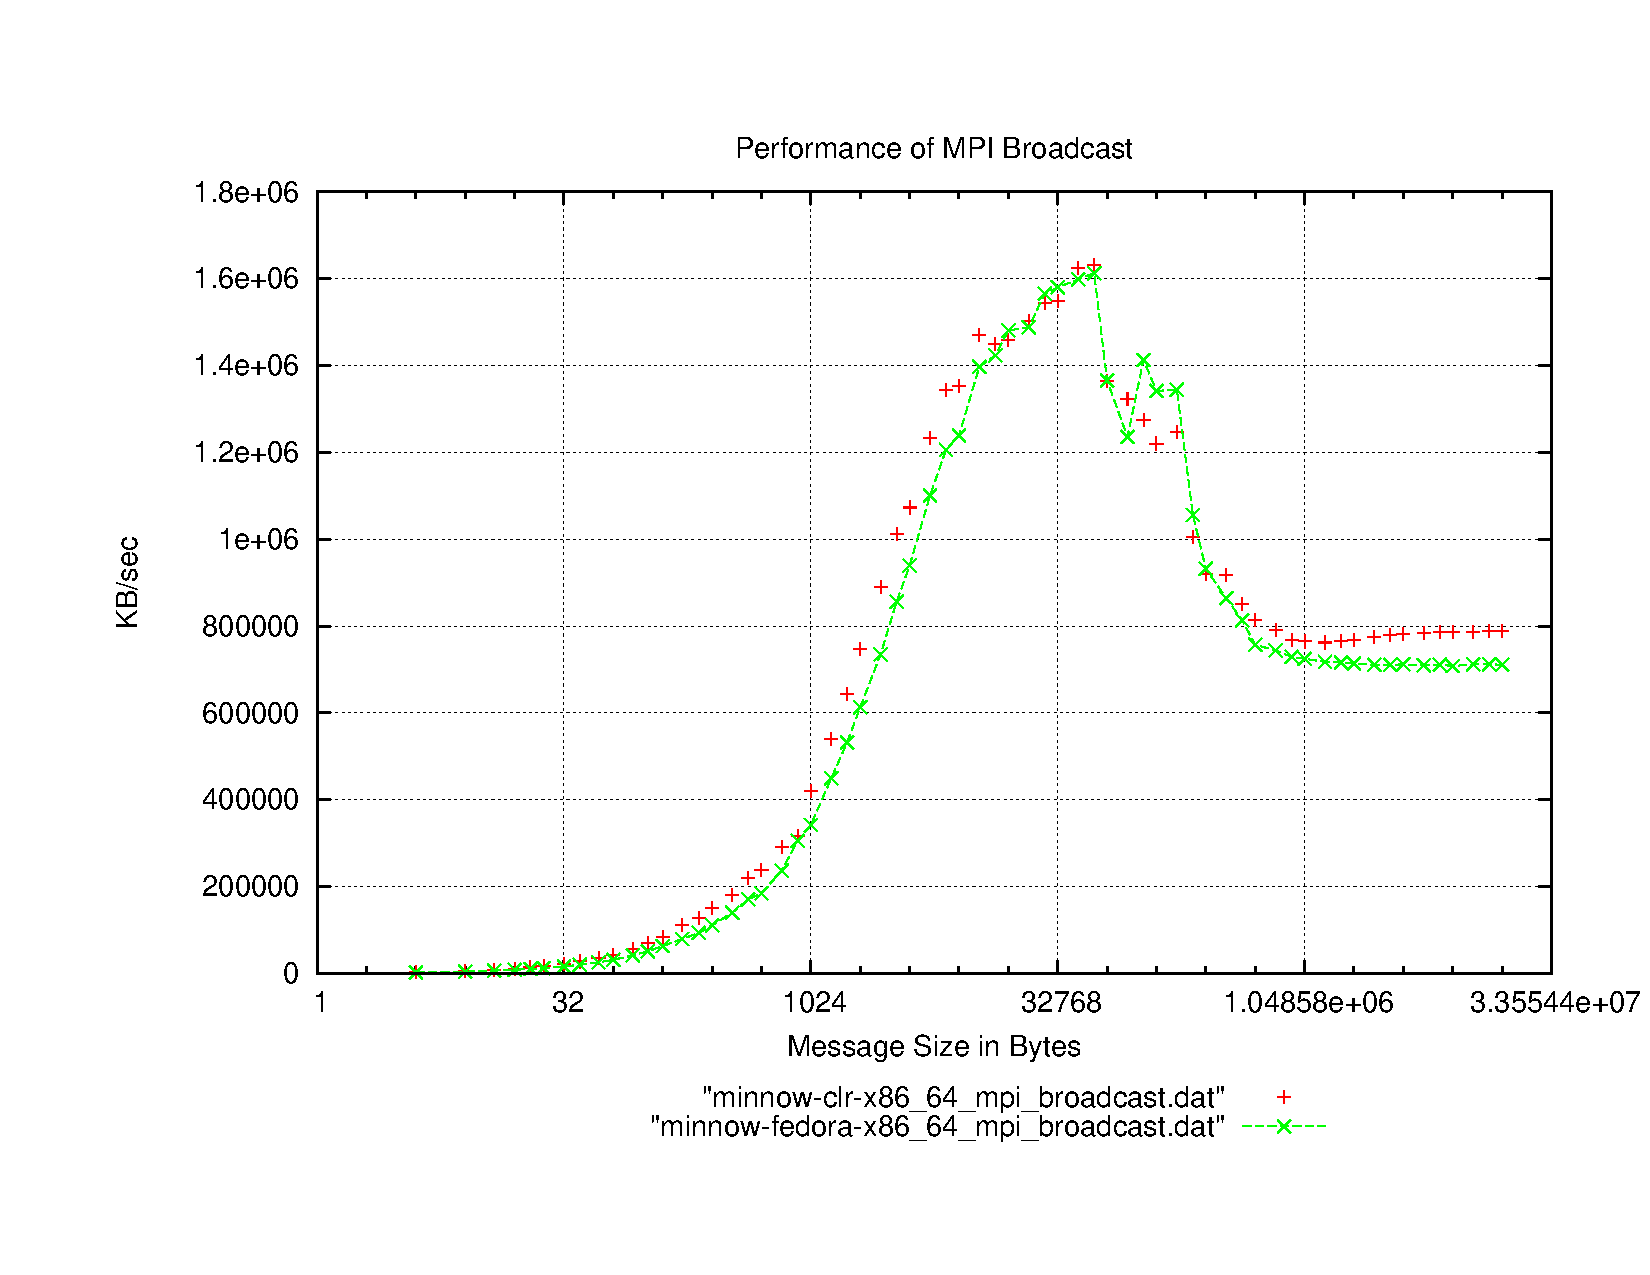
\includegraphics[width=0.75\textwidth]{images/mpbench_clr_experiments/mpi_broadcast.pdf}
\caption{MPI broadcast benchmark running in Minnowboard with Clear Linux and
Fedora (higher is better)}
\label{fig:5.4}
\end{figure}

\begin{figure}[H]
\centering
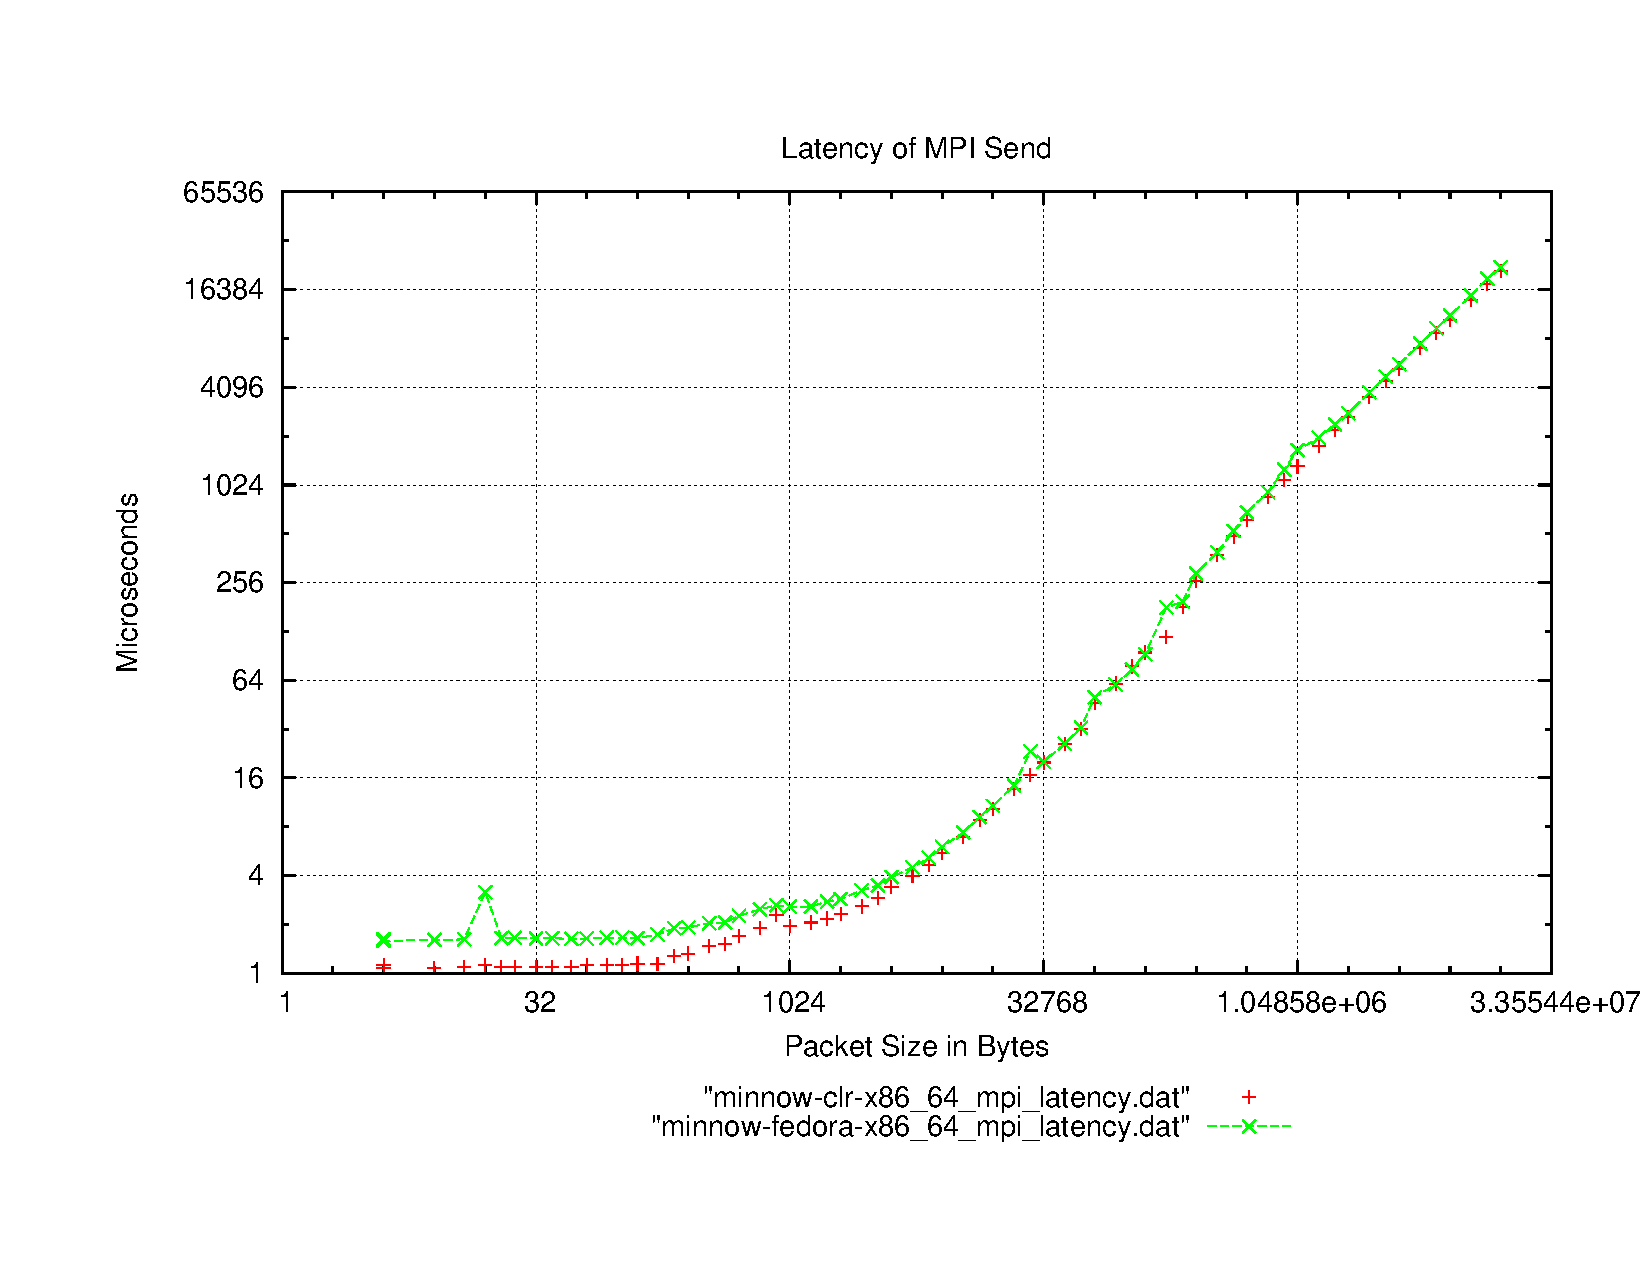
\includegraphics[width=0.75\textwidth]{images/mpbench_clr_experiments/mpi_latency.pdf}
\caption{MPI latency benchmark running in Minnowboard with Clear Linux and
Fedora (lower is better)}
\label{fig:5.5}
\end{figure}

\begin{figure}[H]
\centering
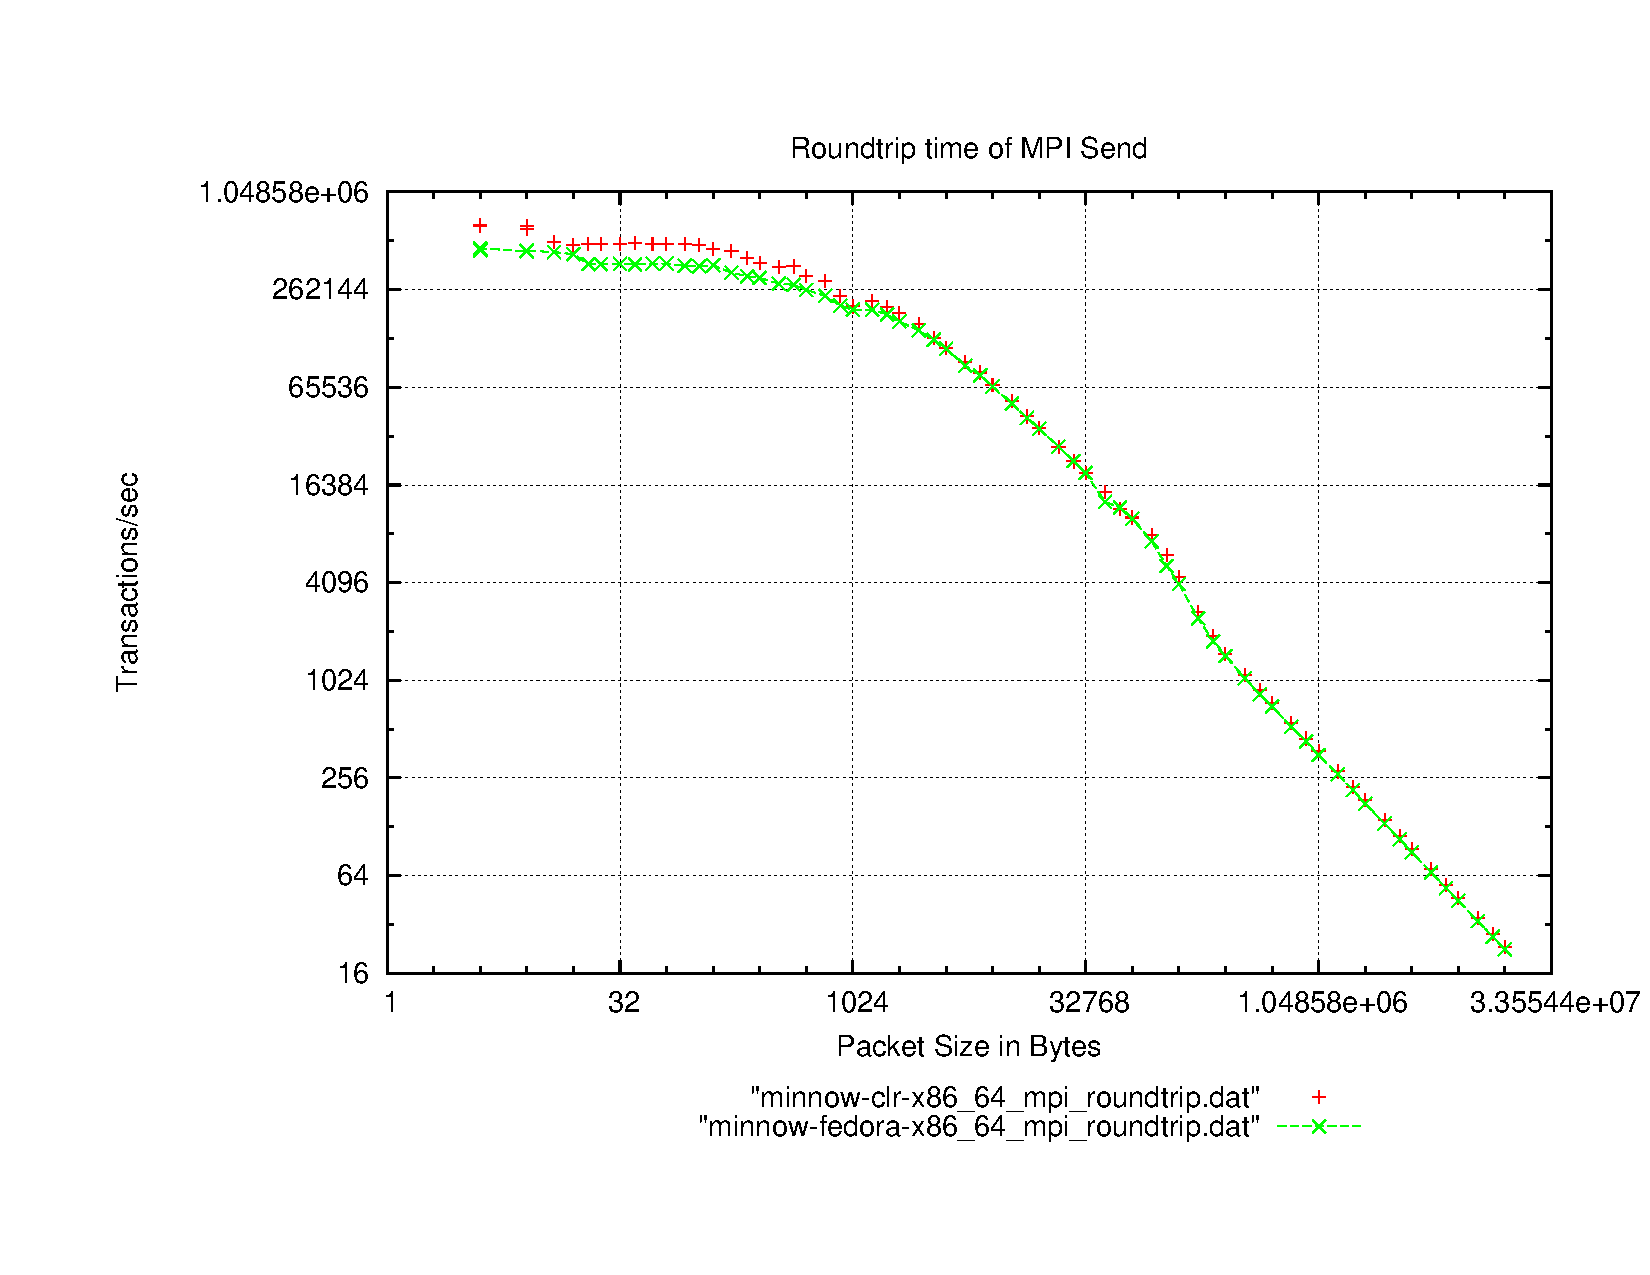
\includegraphics[width=0.75\textwidth]{images/mpbench_clr_experiments/mpi_roundtrip.pdf}
\caption{MPI latency benchmark running in Minnowboard with Clear Linux and
Fedora (lower is better)}
\label{fig:5.6}
\end{figure}

As we know the standard of the industry to generate a custum Linux OS is the
Yocto project. As we saw in table~\ref{tab:4.2} the operating systems generated
with the Yocto project do not have an implementation of the MPI library. Becase
of that we decided to make the MPI implementation in the Yocto project. 


\section{Yocto project MPI implementation}

The Yocto project \cite{yocto-project} generate a custum Linux OS for you
embedded system. The way you add a new capability to the system is by adding a
new receipt. This is described in the Yocto documenttion. The receipt we
implemented for MPI is: 

\begin{lstlisting}[frame=single,numbers=left,breaklines=true]
SUMMARY = "Message Passing Interface (MPI) implementation"
HOMEPAGE = "http://www.mpich.org/"
SECTION = "devel"

LICENSE = "BSD-2-Clause"
LIC_FILES_CHKSUM = "file://COPYRIGHT;md5=2106f0435056f3dd9349747a766e5816"

SRC_URI = " \
	http://www.mpich.org/static/downloads/${PV}/mpich-${PV}.tar.gz \
"

SRC_URI[md5sum] = "40dc408b1e03cc36d80209baaa2d32b7"
SRC_URI[sha256sum] = "455ccfaf4ec724d2cf5d8bff1f3d26a958ad196121e7ea26504fd3018757652d"

CACHED_CONFIGUREVARS += "BASH_SHELL=${base_bindir}/bash"

RDEPENDS_${PN} += "bash perl libxml2"
S = "${WORKDIR}/${BP}"

EXTRA_OECONF = "--enable-debuginfo \
                --enable-fast \
                --enable-shared  \
                --with-pm=gforker  \
		--disable-rpath \
                --disable-f77 \
                --disable-fc \
                --disable-fortran \
                --disable-cxx"

inherit autotools-brokensep gettext

do_configure_prepend() {
    autoreconf --verbose --install --force -I . -I confdb/ -I maint/
    oe_runconf
    exit
}

\end{lstlisting}

This receipt is part of the meta-openembedded layer, (
\url{http://cgit.openembedded.org/cgit.cgi/meta-openembedded/tree/meta-oe/recipes-devtools/mpich/mpich_3.1.1.bb?h=master})
a layer for all the embedded tools that the Linux distros mught need , in this
layer the user can add editors and other libraries that the embedded
application might need. 

The core of the MPI implementation we did is the configure part. Our configure
is described in the ''EXTRA\_OECONF''. The reasons why we did this are : 

\begin{itemize}
\item enable-debuginfo: For debugging the system when nedded
\item enable-fast Turns off error checking and collection of internal timing
information
\item enable-shared;Enable shared library support in order to split the MPI
capabilities in multiple binaries and shared object libraries . This makes the
compiler and process manager applications smaller in size.
\item with-pm=gforker:The gforker process manager is primiarily intended as a
debugging aid as it simplifies development and testing of MPI programs on a
single node or processor.
\item disable-rpath : Do not link to static libraries, if so the build
applications generated by this MPI implementations will not run in other MPI
system with different path of the libraries.
\item disable-f77:Build the Fortran 77 bindings (enabled by default).
\item disable-fc : Build the Fortran 90 bindings (enabled by default), since we
are not supporting Fortran we need to disable it 
\item disable-fortran: We need to disable fortran because Yocto project does
not suport Fortran
\item disable-cxx: Build the C++ bindings (enabled by default). We will not
support C++ in order to generate a small MPI implementation
\end{itemize}

With this configuration we could create an MPI implementation in the Yocto
project, not just the compiler but also the MPI process manager. The results of
doin this can be seen in the following graphs.


\begin{figure}[H]
\centering
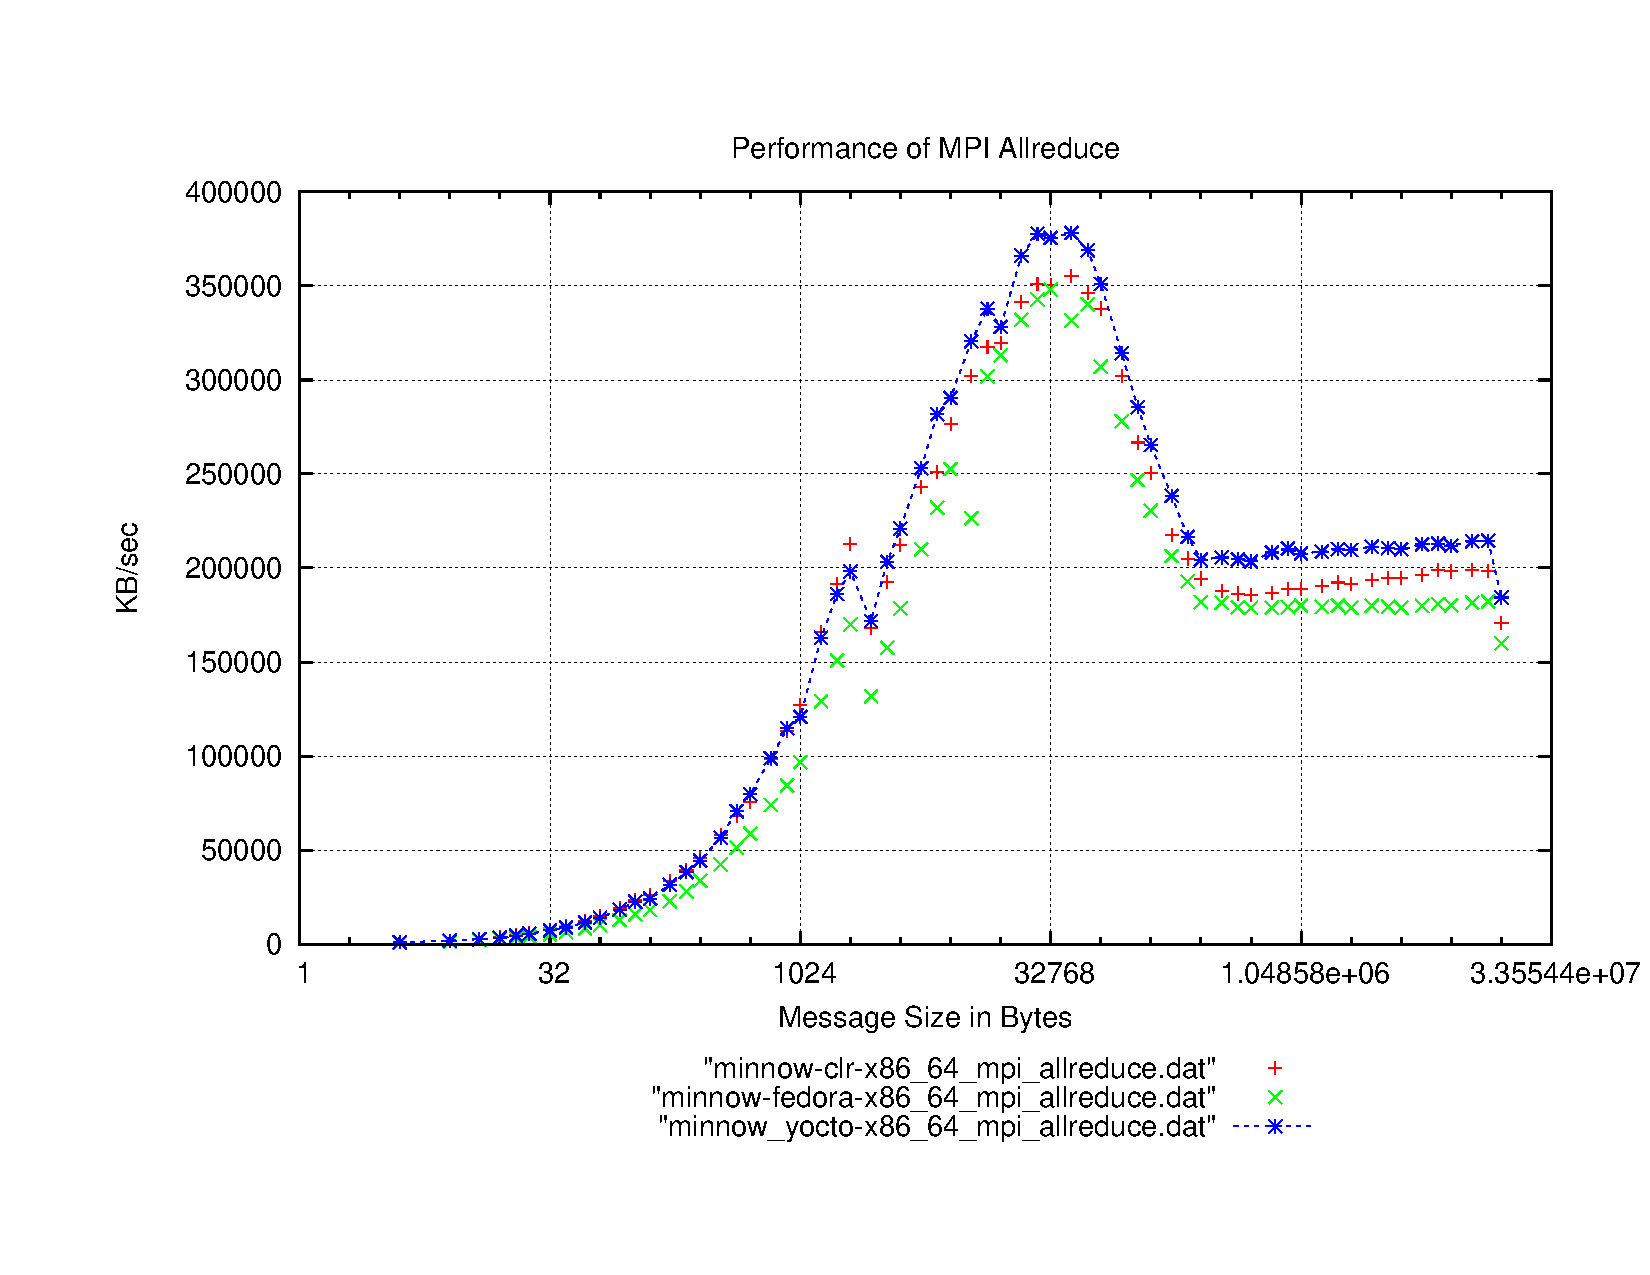
\includegraphics[width=0.75\textwidth]{images/mpbench_yocto_experiments/mpi_allreduce.pdf}
\caption{MPI all reduce benchmark running in Minnowboard with Clear Linux,
Yocto and Fedora (higher is better)}
\label{fig:5.7}
\end{figure}



\begin{figure}[H]
\centering
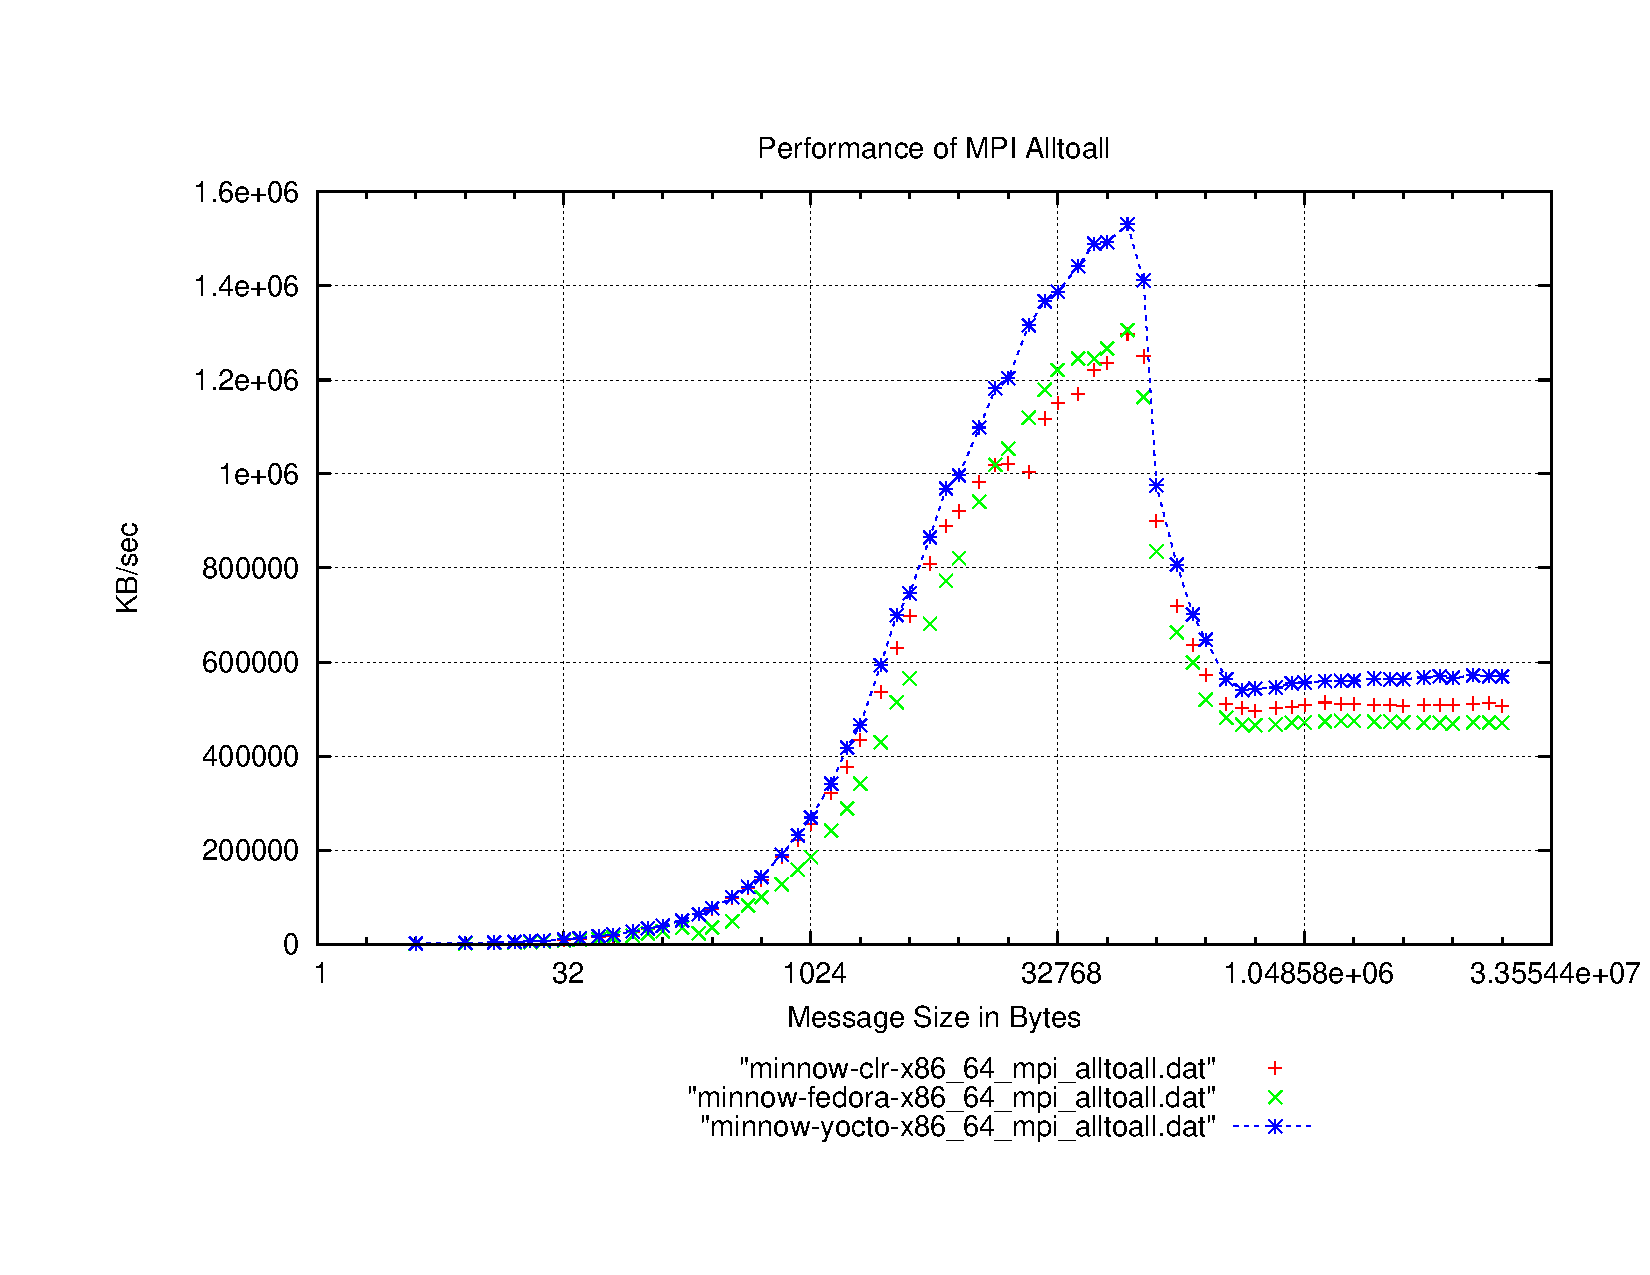
\includegraphics[width=0.75\textwidth]{images/mpbench_yocto_experiments/mpi_alltoall.pdf}
\caption{The Minnow board Max}
\caption{MPI all to all benchmark running in Minnowboard with Clear Linux, Yocto
and Fedora (higher is better)}
\label{fig:5.8}
\end{figure}


\begin{figure}[H]
\centering
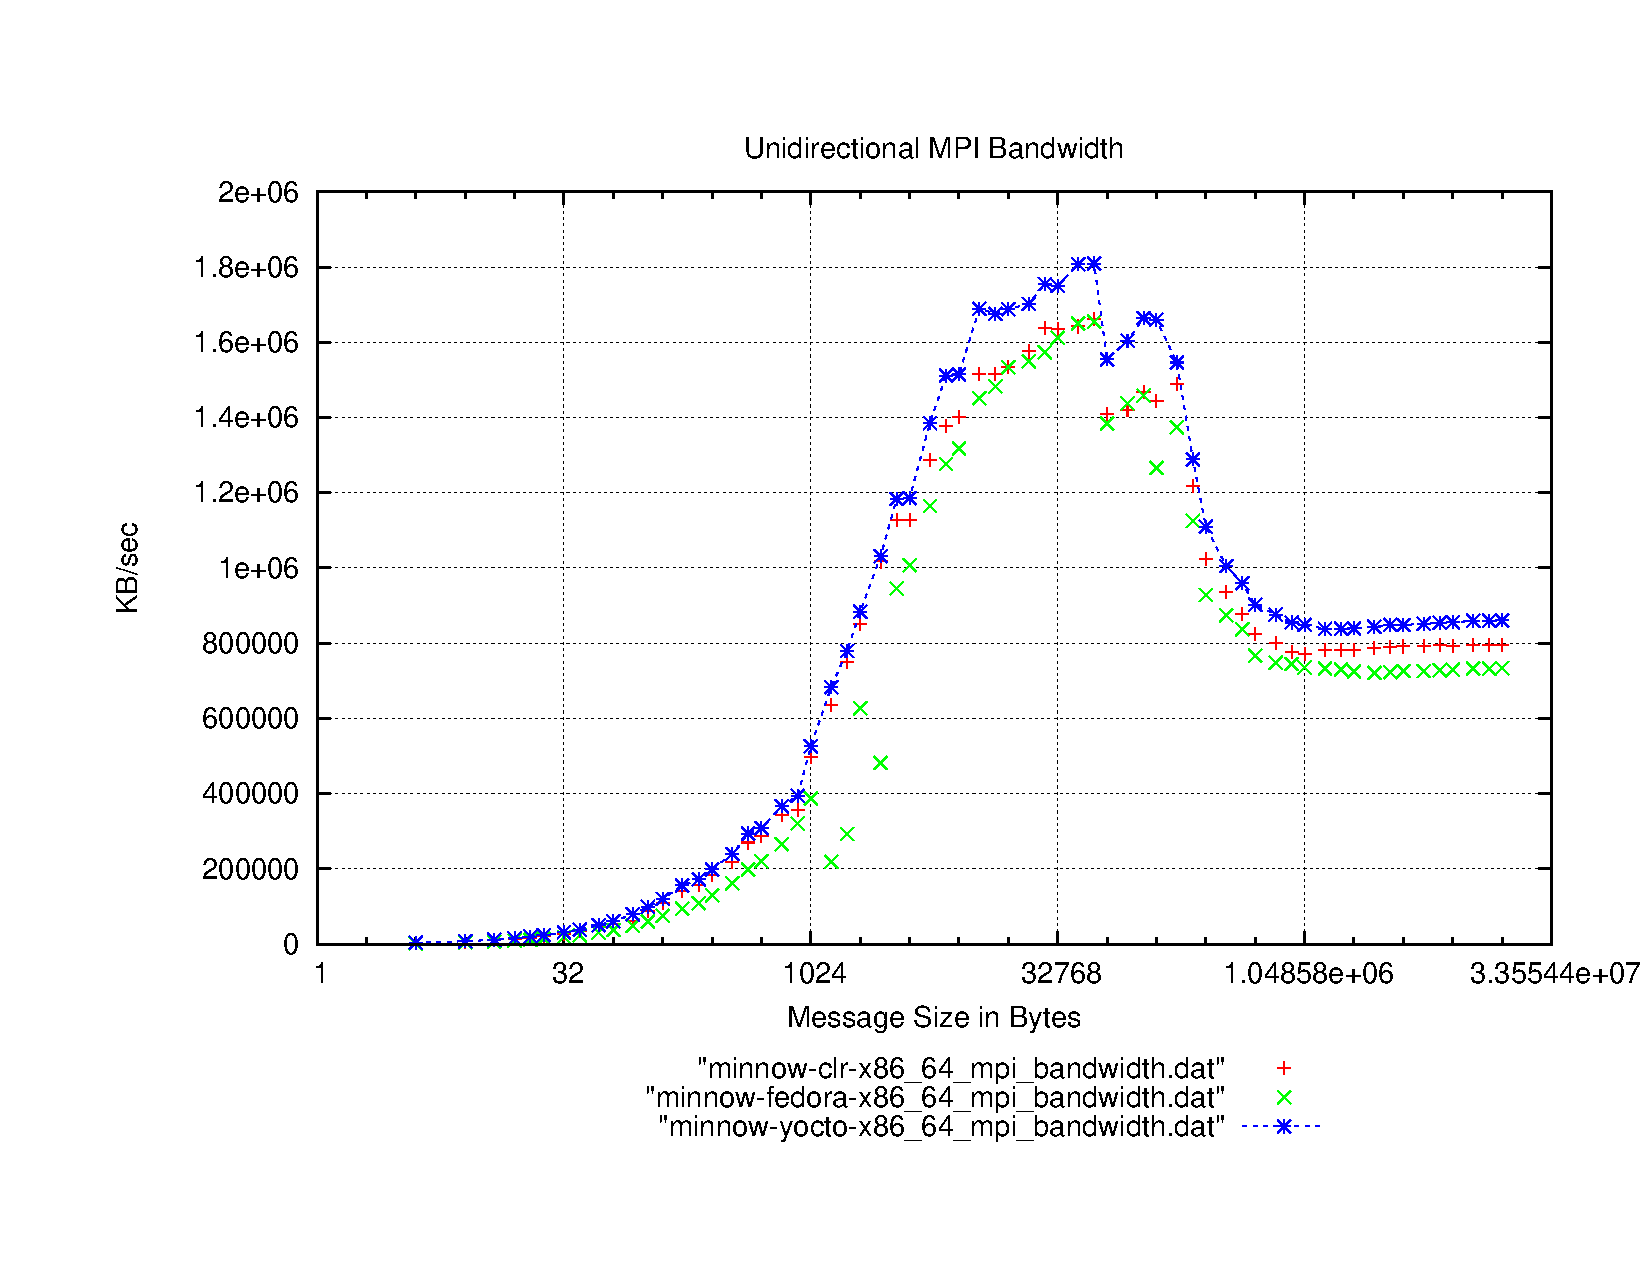
\includegraphics[width=0.75\textwidth]{images/mpbench_yocto_experiments/mpi_bandwidth.pdf}
\caption{The Minnow board Max}
\caption{MPI bandwidth benchmark running in Minnowboard with Clear Linux,
Yocto and Fedora (higher is better)}
\label{fig:5.9}
\end{figure}


\begin{figure}[H]
\centering
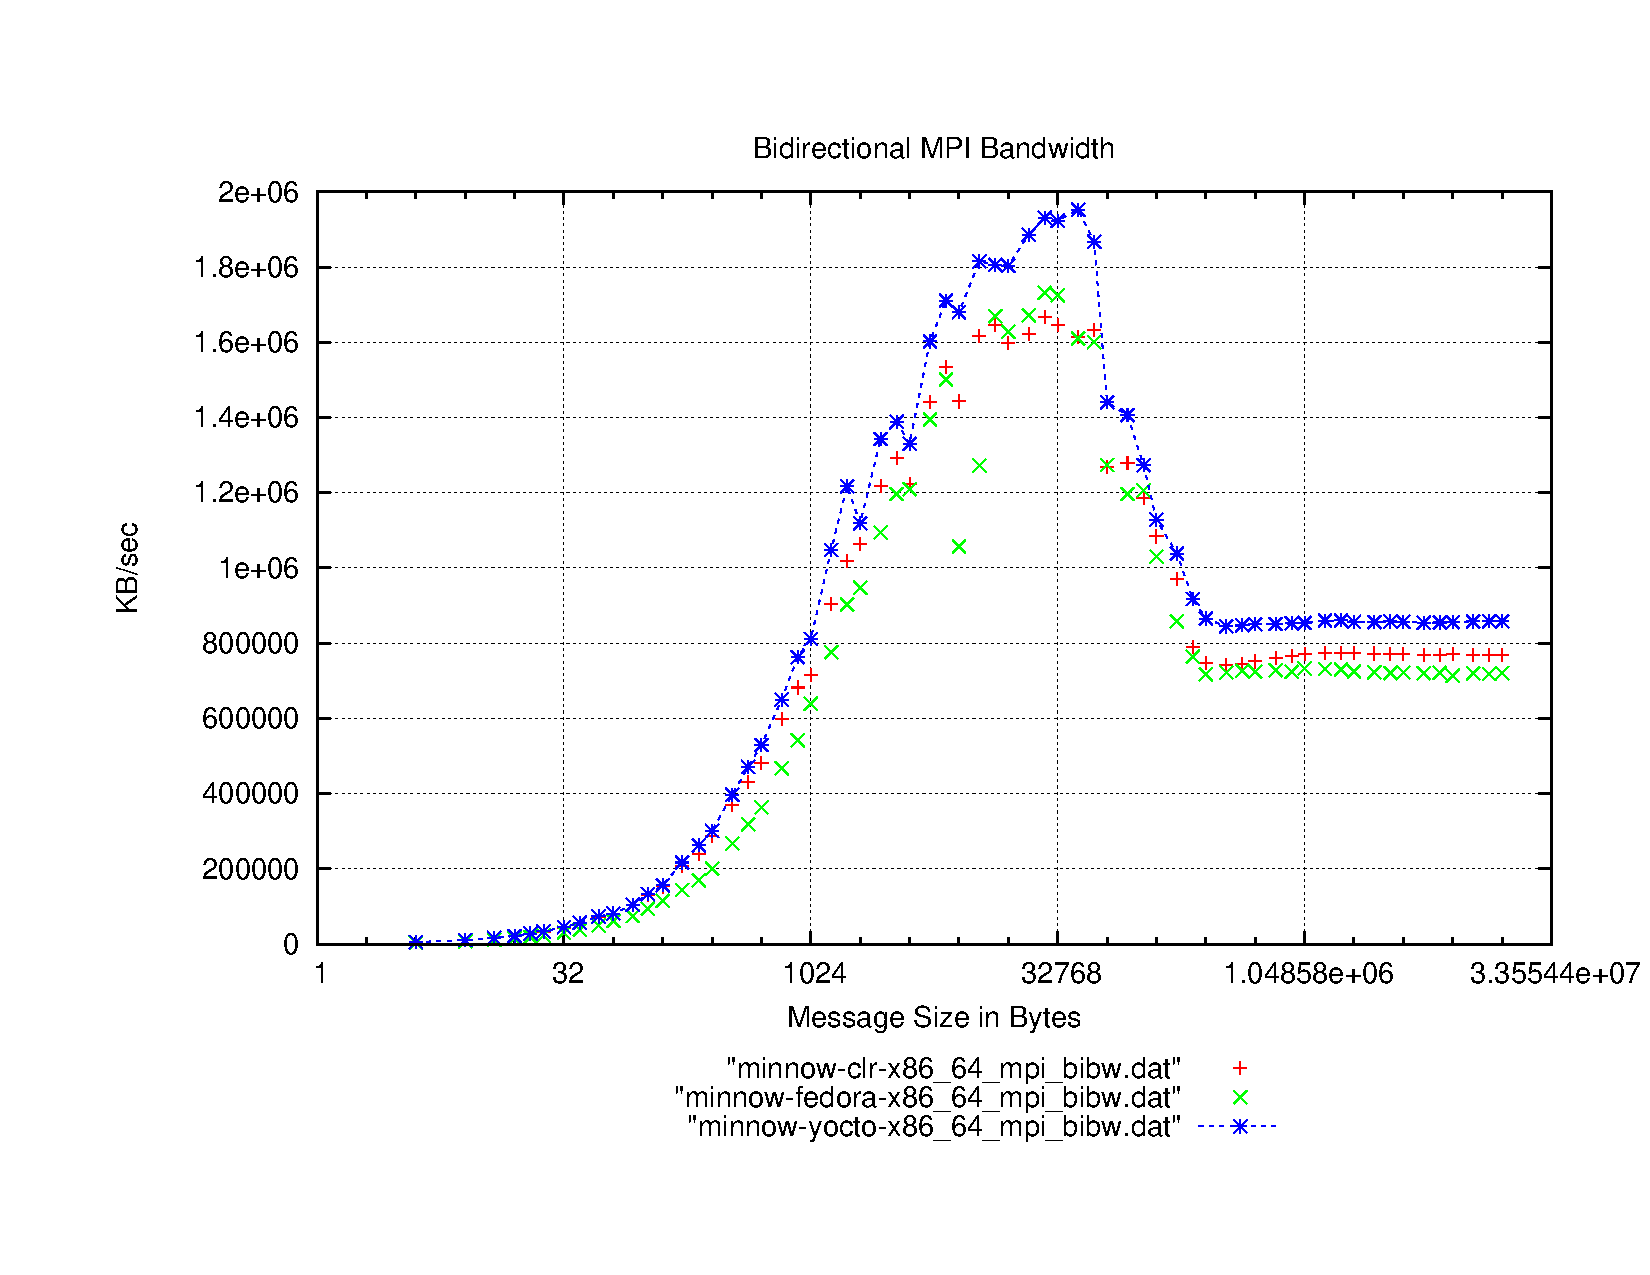
\includegraphics[width=0.75\textwidth]{images/mpbench_yocto_experiments/mpi_bibw.pdf}
\caption{The Minnow board Max}
\caption{MPI Bi directional bandwidth running in Minnowboard with Clear Linux,
Yocto and Fedora (higher is better)}
\label{fig:5.10}
\end{figure}


\begin{figure}[H]
\centering
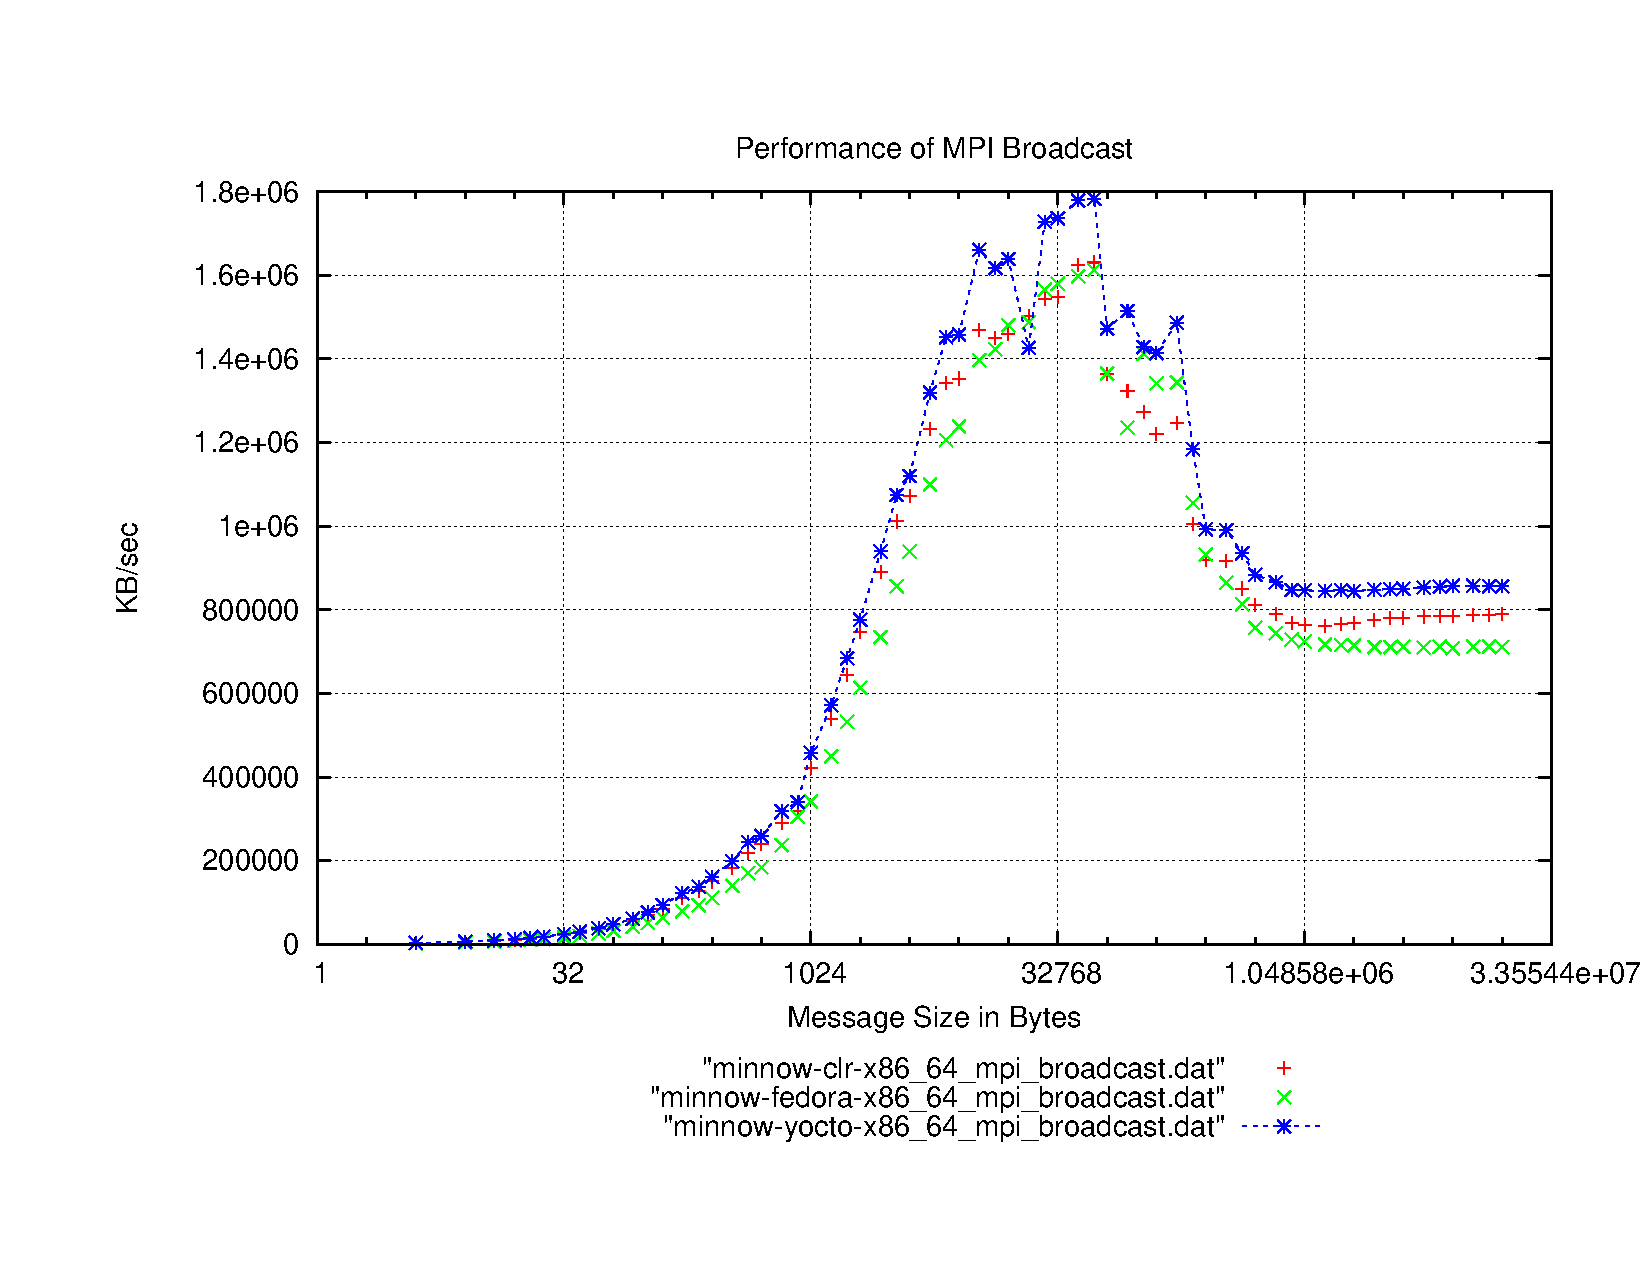
\includegraphics[width=0.75\textwidth]{images/mpbench_yocto_experiments/mpi_broadcast.pdf}
\caption{The Minnow board Max}
\caption{MPI Broadcast benchmark running in Minnowboard with Clear Linux, Yocto
and Fedora (lower is better)}
\label{fig:5.11}
\end{figure}

\begin{figure}[H]
\centering
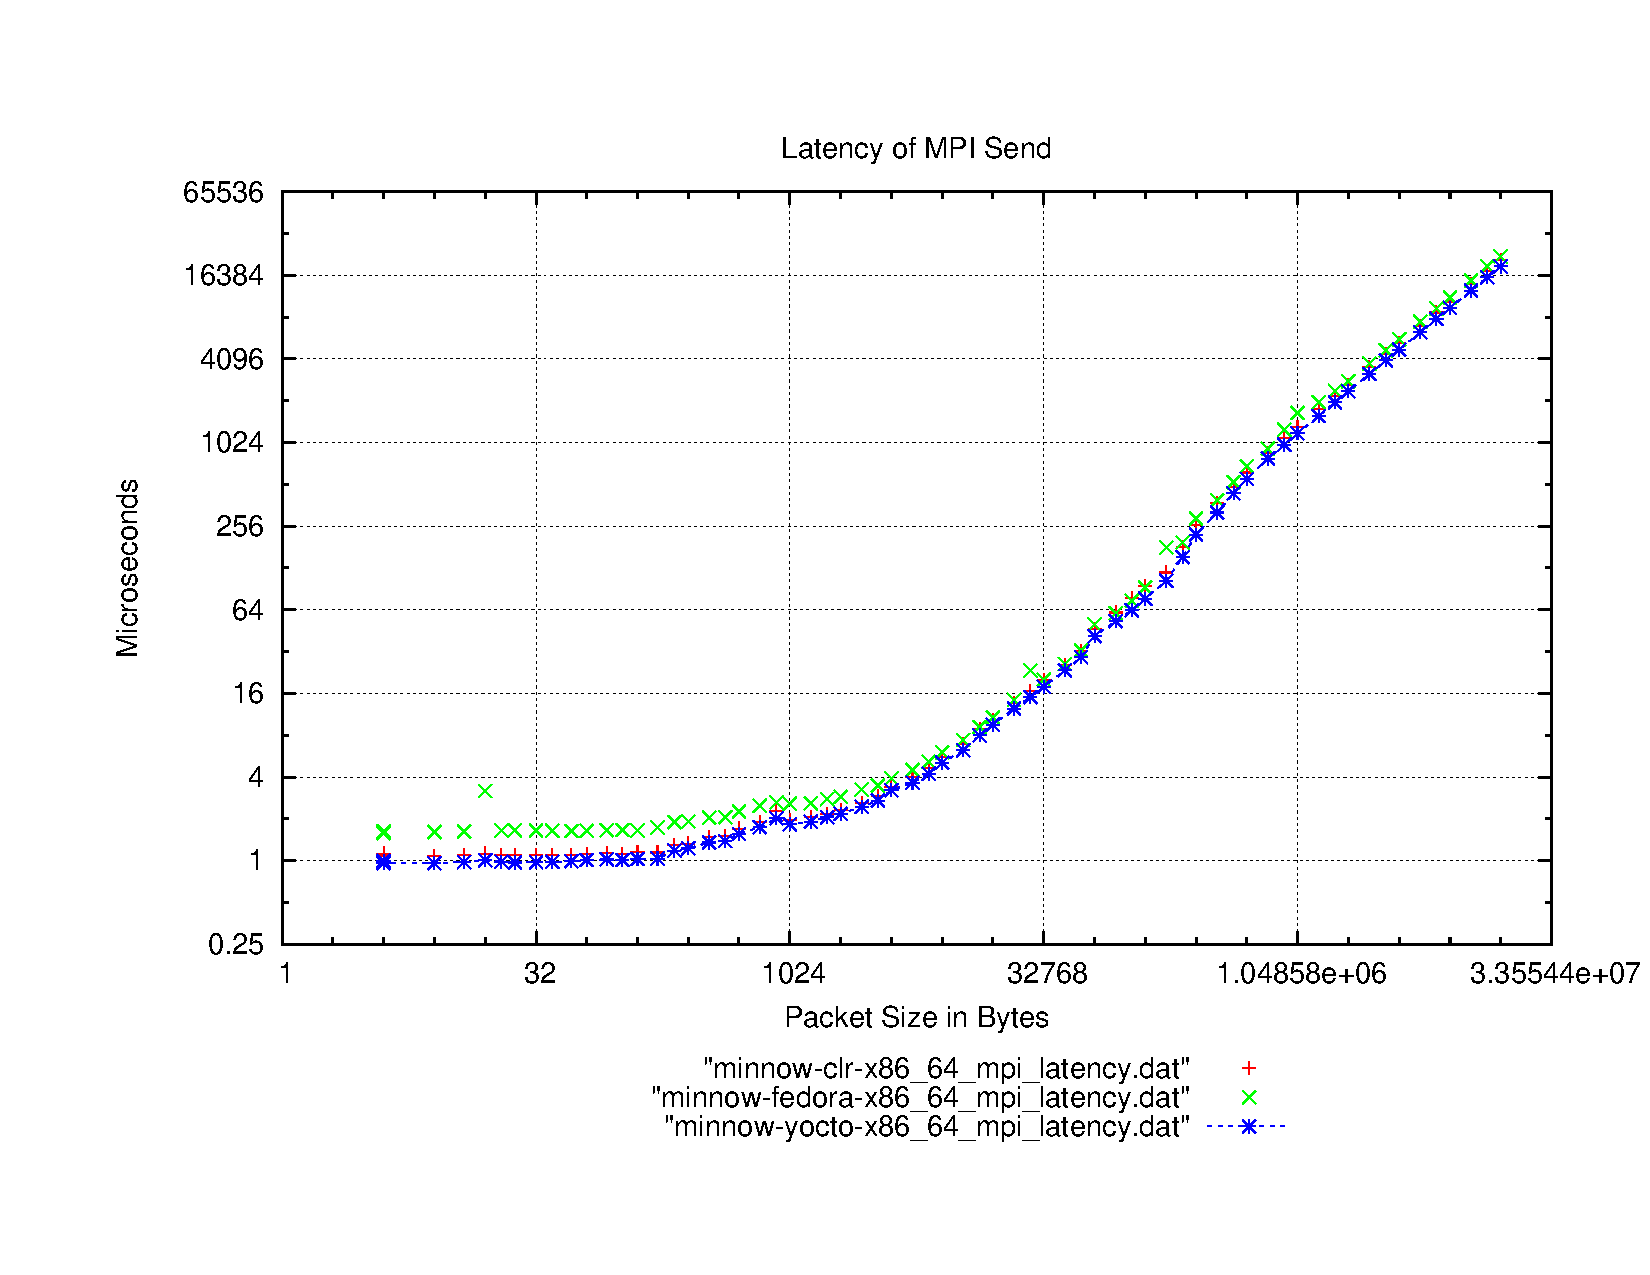
\includegraphics[width=0.75\textwidth]{images/mpbench_yocto_experiments/mpi_latency.pdf}
\caption{MPI latency running in Minnowboard with Clear Linux,
Yocto and Fedora (higher is better)}
\label{fig:5.12}
\end{figure}

\begin{figure}[H]
\centering
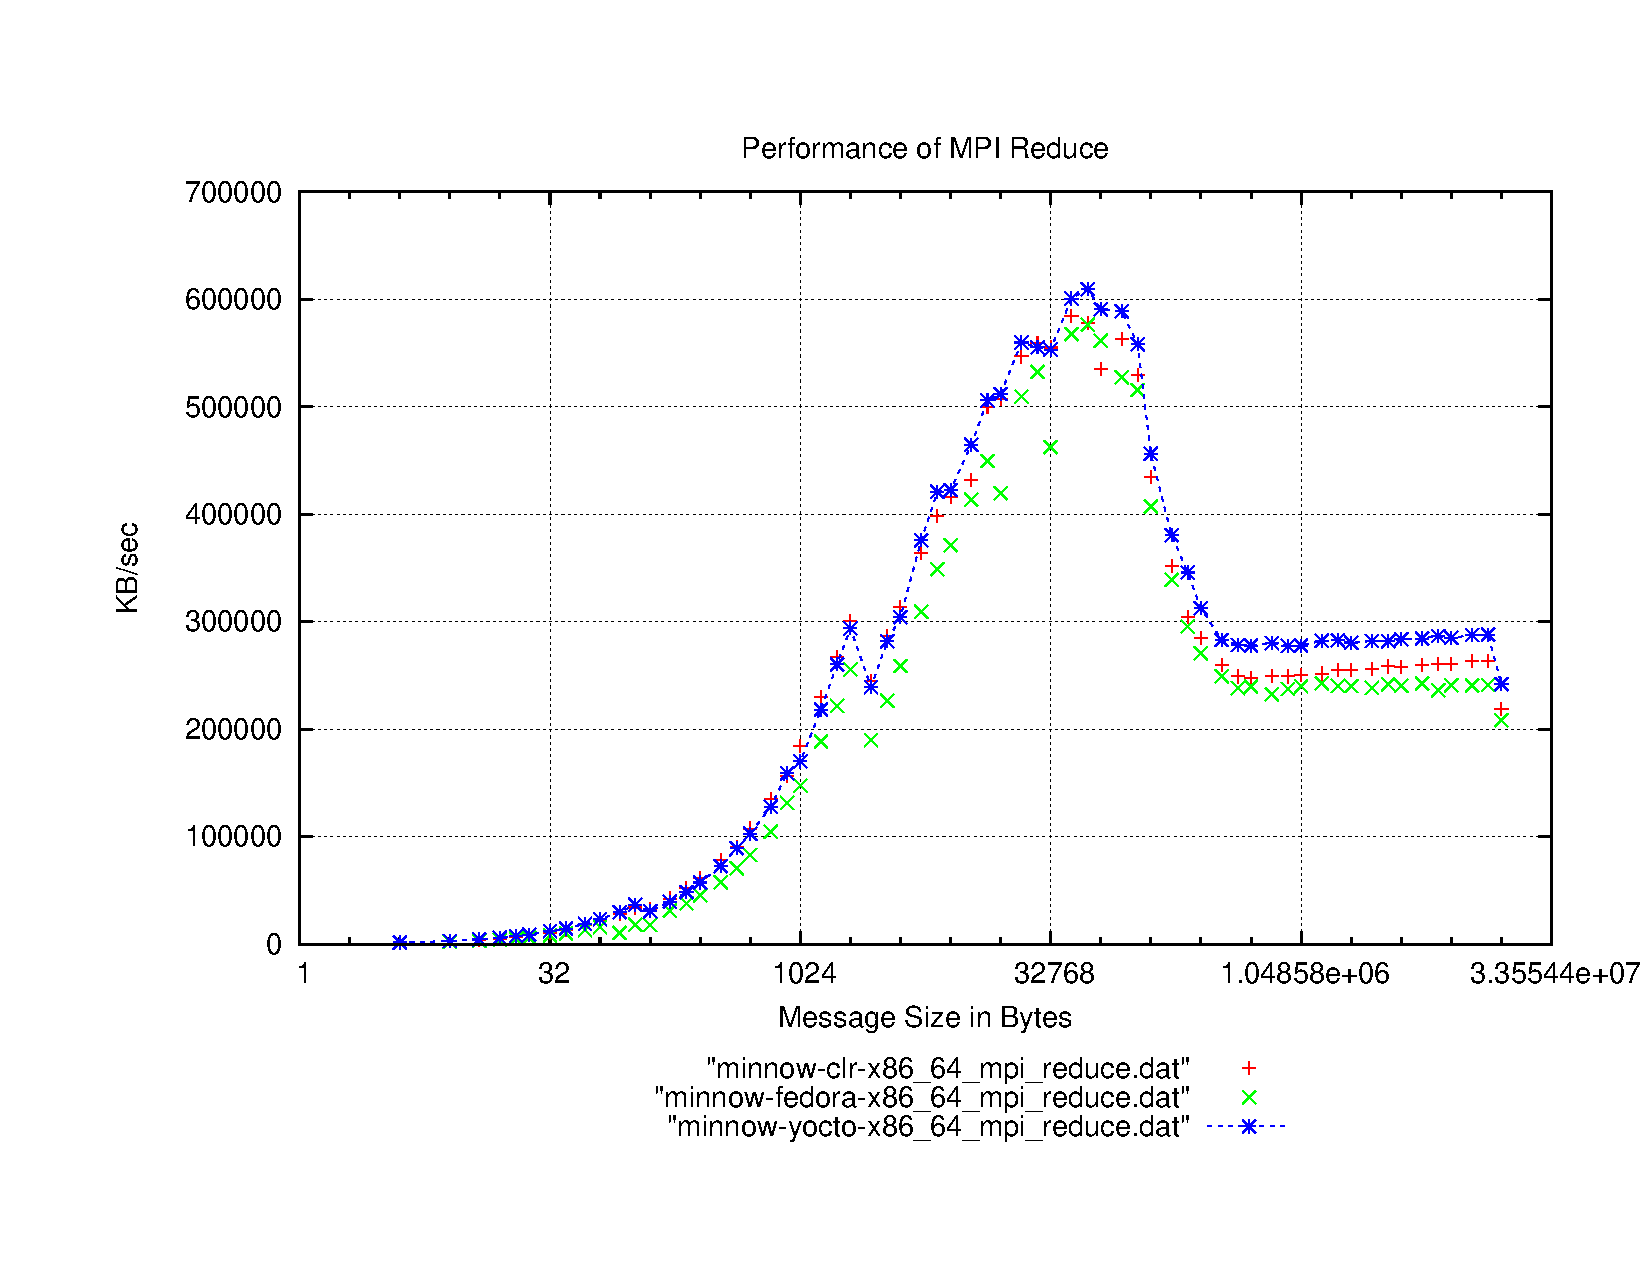
\includegraphics[width=0.75\textwidth]{images/mpbench_yocto_experiments/mpi_reduce.pdf}
\caption{MPI Reduce benchmark running in Minnowboard with Clear Linux, Yocto
and Fedora (higher is better)}
\label{fig:5.13}
\end{figure}

\begin{figure}[H]
\centering
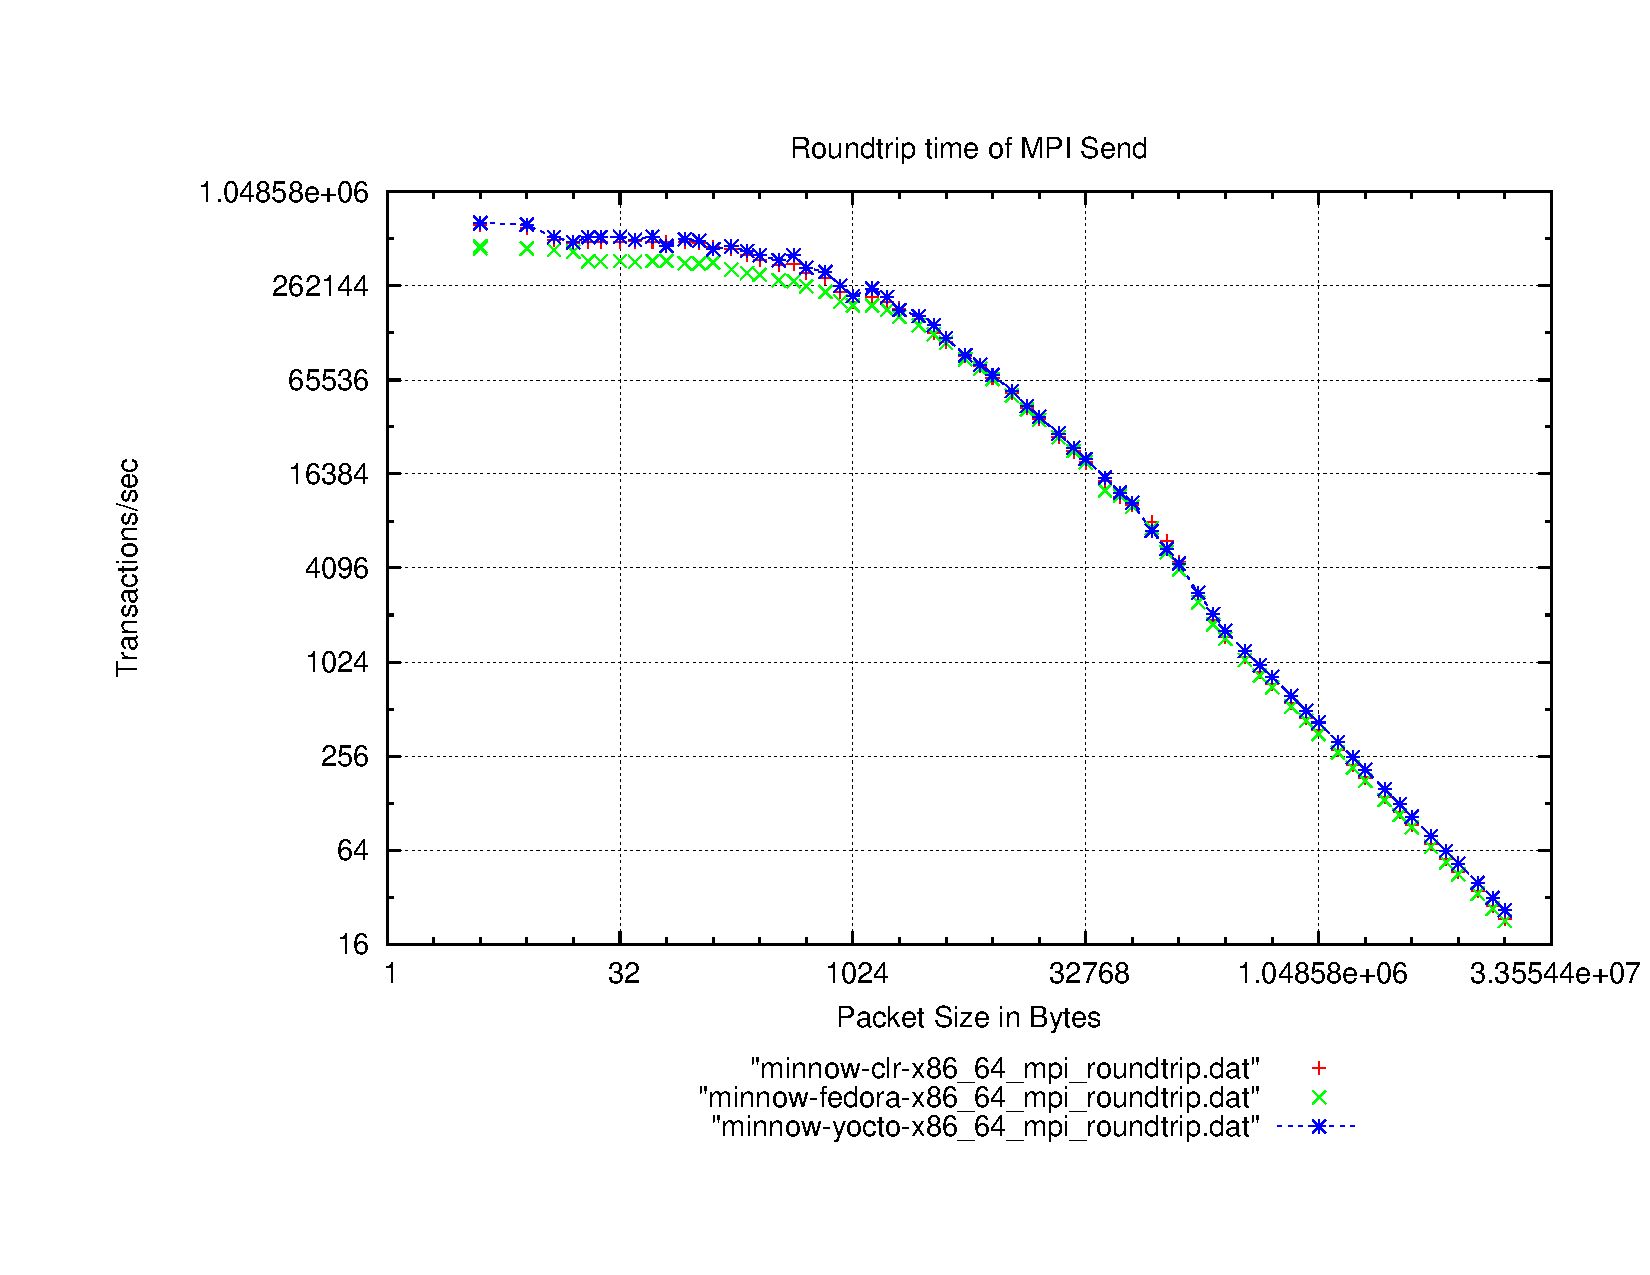
\includegraphics[width=0.75\textwidth]{images/mpbench_yocto_experiments/mpi_roundtrip.pdf}
\caption{MPI Bi directional bandwidth running in Minnowboard with Clear Linux,
Yocto and Fedora (lower is better)}
\label{fig:5.14}
\end{figure}


\section{Test MPI benchmark in a cluster of embedded systems}

\section{Test MPI benchmark in a cluster of embedded systems}

\section{Test MPI benchmark in a cluster of embedded systems}
\clearpage
